\section{Building the Monte-Carlo Prediction}
T2K has been taking data since 2010 with steadily increasing beam power and protons on target (POT), and is currently on ``run 9'', shown earlier in \autoref{fig:t2k_pot}. This analysis uses data from runs 2 to 6: run 1 was omitted because parts of the detector was uninstrumented (and is only $\sim4\%$ of the run 1-6 data), and run 7 and beyond had not gone through full Monte-Carlo production until summer 2017. 

The overall efficiency of ND280 in runs 2 to 6 was approximately 85\%, collecting 9.7E20 POT out of 12E20 POT. The good POT\footnote{Defined as POT collected when all ND280 sub-detectors and global DAQ are flagged online} per run used in this analysis is listed in \autoref{tab:pot_2017}.

\begin{table}[h]
	\centering
	\begin{tabular}{ l | c c c }
		\hline
		Run & Data POT (E19) & MC POT (E19) & Sand POT (E19) \\
		\hline
		\hline
		2a  FHC & 3.59337    & 92.15       & 10 \\
		2w  FHC & 4.33934    & 120.15      & 10 \\
		\hline
		3b FHC  & 2.17273    & 44.8        & 5 \\
		3c FHC  & 13.6447    & 263         & 25 \\
		\hline
		4a FHC  & 17.8271    & 349.9       & 30 \\
		4w FHC  & 16.4277    & 349.65      & 29.15 \\
		\hline
		5 RHC & 4.3468     & 208.25      & 20 \\
		\hline
		6b RHC & 12.8838    & 141.03      & 40 \\
		6c RHC & 5.07819    & 53.21       & 15 \\
		6d RHC & 7.75302    & 69.41       & 20 \\
		6e RHC & 8.51668    & 86.72       & 23 \\
		\hline
		\hline
		Total FHC & 58.00494 & 1219.65 & 109.15\\
		Total RHC & 38.57849 & 558.62  & 118 \\
		\hline
		Total & 96.58343 & 1778.27 & 227.15 \\
		\hline
	\end{tabular}
	\caption{Counted and generated proton-on-targets for the T2K ND280 2017 analysis}
	\label{tab:pot_2017}
\end{table}
The Monte-Carlo is generated for the different run-periods to account for beam configurations, ND280 configurations, run-dependent calibrations, and so on. Runs marked ``a'' and ``w'' refer to the P0D detector's removable water bags being air filled (a) or water filled (w), which require different ND280 geometries in the simulation.

To build the nominal distribution for direct comparison to data, a number of scalings and weights are applied. For the ND280 analysis all weights are applied on an event-by-event basis\footnote{Which is not the case for SK analyses}:
\begin{itemize}
	\item \textbf{POT weight:} \\
	A run-by-run scaling factor taking the ratio of total good flagged data to the generated Monte-Carlo POT. An event receives a one-time weight depending on what run it was from and how much MC was generated in the production. These numbers can be read off directly from \autoref{tab:pot_2017}. This weight $w_\text{POT}$ is only applied once and is not varied in the fit.
	
	\item \textbf{Flux weight:} \\
	A run-by-run correction to the nominal neutrino flux which the full experiment simulation was made in. The weight is applied as a function of $E_\nu^{true}$ with~$0 < E_\nu^{true} < 30 \text{ GeV}$~, detailed in \autoref{subsec:syst_flux}. An event receives a weight depending on what run it was from and its $E_\nu^{true}$. The weight $w_\text{Flux}$ is only applied once and is not varied in the fit.
	
	\item \textbf{Beam variation weight:} \\
	An event-by-event weight to vary the impact of the flux simulation. An event gets weighted as a function of the neutrino run, the flavour of neutrino ($\nu_\mu$, $\bar{\nu}_\mu$, $\nu_e$ or $\bar{\nu}_e$) and the neutrino energy, detailed in \autoref{subsec:syst_flux}.
	
	The weight $w_{\vec{b}\rightarrow \vec{b}'}$ is applied once to weight the simulation to nominal, and is recalculated for every iteration of the fit.
	
	\item \textbf{Cross-section variation weight:} \\
	An event-by-event weight taking the full generated event through the neutrino interaction simulation, calculating a weight to apply to the event. The applied weight is pre-calculated as $w_{\vec{x} \rightarrow \vec{x}'}=\sigma(\vec{x}')/\sigma(\vec{x})$ for the generated neutrino interaction systematic parameter values $\vec{x}$ and the modified parameter values $\vec{x}'$. The event can receive a normalisation and a shape parameter depending on its interaction type and the interaction model considered in the analysis, detailed in \autoref{subsec:syst_xsec}.
	
	The weight $w_{\vec{x}\rightarrow \vec{x}'}$ is applied once to weight the simulation to nominal, and is recalculated for every iteration of the fit.
	
	\item \textbf{Detector variation weight:} \\
	An event-by-event weight from the reconstruction and selection package to vary the impact of the detector simulation. It is applied as a function of the event's topology and detector (e.g. FGD1 CC0$\pi$), its \pmu and \cosmu. The weights are normalisation parameters $\vec{d}$ for each bin in the detector covariance matrix, explained in detail in \autoref{subsec:syst_nd280}.
	
	The weight $w_{\vec{d}\rightarrow \vec{d}'}$ is applied once to weight the simulation to nominal, and is recalculated for every iteration of the fit.
\end{itemize}

All weights are parameterised as multiplicative, so for a two parameter variation $x \rightarrow x'$ and $y \rightarrow y'$ we have the total weight 
\begin{equation}
w_{x \rightarrow x', y \rightarrow y'} = w_{x \rightarrow x', y \rightarrow y} \times w_{x \rightarrow x, y\rightarrow y'}
\end{equation}

Defining the beam parameters as $\vec{b}$, cross-section parameters as $\vec{x}$ and detector parameters as $\vec{d}$, we express one rescaled Monte-Carlo event $\lambda_i$ as

\begin{equation}
\lambda_i\left(\vec{b}, \vec{x}, \vec{d}\right) = 1 \times w_i^\text{POT} \times w_i^\text{Flux} \times w^{\vec{b}\rightarrow \vec{b}'}_i \times w^{\vec{x} \rightarrow \vec{x}'}_i \times w^{\vec{d}\rightarrow \vec{d}'}_i
\label{eq:mc_scale}
\end{equation}

The effect of each weight on the predictions for each ND280 selection is shown in \autoref{tab:eventrate_mach3}. The nominal flux and detector weights are 1.0, so are not included in the table.
\begin{sidewaystable}
	\centering
	\begin{tabular}{ l | c | c | c | c | c }
		\hline
		Sample & Raw MC & POT only & POT+xsec & POT+NDCov & POT+BeamCov \\ 
		\hline
		\hline
		\FGDCCNoPi{1}{\numu}& 337436 & 15905.2 & 15340.2 & 16246.1 & 16090.8 \\
		\FGDCCOnePi{1}{\numu}& 84982  & 4011.58 & 3819.3 & 4131.35 & 4058.36 \\
		\FGDCCOther{1}{\numu}& 65286 & 3071.21 & 3078.52 & 3374.21 & 3107.04 \\
		\FGDCCNoPi{2}{\numu}& 345467 & 16259.6 & 15749.8 & 16415 & 16449.2 \\
		\FGDCCOnePi{2}{\numu}& 70444  & 3318.26 & 3190.09 & 3321.4 & 3356.97 \\
		\FGDCCOther{2}{\numu}& 63402  & 2983.43 & 2995.68 & 3051.48 & 3018.22 \\
		\FGDCCOneTrk{1}{\numubar}& 54419  & 3744.02 & 3430.15 & 3872.18 & 3773.79 \\
		\FGDCCNTrk{1}{\numubar}& 15392  & 1056.8 & 986.32 & 1121.1 & 1065.2 \\
		\FGDCCOneTrk{2}{\numubar}& 55732  & 3833.73 & 3506.36 & 3906.32 & 3864.24 \\
		\FGDCCNTrk{2}{\numubar}& 15808  & 1088.15 & 1024.77 & 1122.73 & 1096.81 \\
		\FGDCCOneTrk{1}{\numu} in RHC& 18146 & 1246.03 & 1194.72 & 1262.00 & 1255.92 \\
		\FGDCCNTrk{1}{\numu} in RHC& 17156 & 1181.54 & 1172.13 & 1257.34 & 1190.94 \\
		\FGDCCOneTrk{2}{\numu} in RHC& 18052 & 1231.24 & 1189.64 & 1245.3 & 1241.02 \\
		\FGDCCNTrk{2}{\numu} in RHC& 16339 & 1127.64 & 1121.37 & 1150.7 & 1136.62 \\
		\hline
		\hline
	\end{tabular}
	\caption{Event rates broken by type of weight applied for the nominal MC samples}
	\label{tab:eventrate_mach3}
\end{sidewaystable}

\section{Nominal Model Prediction}
\label{sec:nom_model}
The rates for the data and nominal model with all mentioned Monte-Carlo scalings and selections are presented in \autoref{tab:event_rates_2017}. We note that generally the Monte-Carlo rates of the CC0$\pi$ and CC1Track are underestimated (2-3\%) , CC$1\pi$ is overestimated (6-11\%) and CCOther is under-estimated (5-15\%). \numubar selections except FGD2 CC1Track \numubar are overestimated by 5\%, with FGD1 being 2\%. The \numu in RHC selections are mildly underestimated. The rates across the FGDs are consistent for all selections.
\begin{table}[h]
	\centering
	\begin{tabular}{ l | c c c }
		\hline
		\hline
		Sample & Data & Nominal MC & Data/MC \\
		\hline
		\FGDCCNoPi{1}{\numu}           & 17136 & 16723.80 & 1.02 \\% \hline
		\FGDCCOnePi{1}{\numu}          & 3954  & 4381.47 & 0.90 \\% \hline
		\FGDCCOther{1}{\numu}          & 4149  & 3943.95 & 1.05\\% \hline
		\hline
		\FGDCCNoPi{2}{\numu}           & 17443 & 16959.30 & 1.03 \\% \hline
		\FGDCCOnePi{2}{\numu}          & 3366  & 3564.23  & 0.94\\% \hline
		\FGDCCOther{2}{\numu}          & 4075  & 3570.94  & 1.14 \\% \hline
		\hline
		\FGDCCOneTrk{1}{\numubar}      & 3527 & 3587.77 & 0.98 \\% \hline
		\FGDCCNTrk{1}{\numubar}   	   & 1054 & 1066.91 & 0.99 \\% \hline
		\hline
		\FGDCCOneTrk{2}{\numubar}      & 3732 & 3618.29 & 1.03 \\% \hline
		\FGDCCNTrk{2}{\numubar}        & 1026 & 1077.24 & 0.95\\% \hline
		\hline
		\FGDCCOneTrk{1}{\numu} in RHC  & 1363 & 1272.17 & 1.07 \\% \hline
		\FGDCCNTrk{1}{\numu} in RHC    & 1370 & 1357.45 & 1.01 \\% \hline
		\hline
		\FGDCCOneTrk{2}{\numu} in RHC  & 1320 & 1262.63 & 1.05 \\% \hline
		\FGDCCNTrk{2}{\numu} in RHC    & 1253 & 1246.71 & 1.01\\% \hline
		\hline
		Total & 64768 & 63632.86 & 0.98 \\\hline
		\hline
	\end{tabular}
	\caption{Observed and predicted event rates for the different ND280 selections for the 2017 analysis}
	\label{tab:event_rates_2017}
\end{table}

\autoref{fig:nominal1D_pmu} shows the projections of the 2D distributions onto \pmu, where we note generally good modelling. The 2D distributions can be found in \autoref{chap:nominal_mc_2017}.

The CC0$\pi$ selections have a clear oscillation from under-prediction to overprediction for FGD1 and FGD2 in $0 < p_\mu < 1 \text{ GeV}$. The FGD1 \numubar CC1Track selection appears to show similar behaviour although without the under-prediction at low \pmu, although FGD2 \numu CC1Track does not. The CC1$\pi$ selection shows a nearly consistent over-estimation of $\sim10\%$ in every bin for both FGDs. The CCOther selection is instead underestimated at the event distribution peak, into the tail ($0.5<p_\mu <1.5\text{ GeV}$). The CCNtrack distributions are consistent with good modelling due to their large statistical errors.
% left bottom right top
\begin{figure}[h]
\begin{subfigure}[t]{0.32\textwidth}
	\includegraphics[width=\textwidth,page=43,trim={0mm 125mm 40mm 0mm},clip]{{figures/mach3/selection/2017b_nominal_withdebug_forthesis_ND280_nom.pdf}}
\end{subfigure}
\begin{subfigure}[t]{0.32\textwidth}
\includegraphics[width=\textwidth,page=43,trim={0mm 55mm 40mm 70mm},clip]{{figures/mach3/selection/2017b_nominal_withdebug_forthesis_ND280_nom.pdf}}
\end{subfigure}
\begin{subfigure}[t]{0.32\textwidth}
\includegraphics[width=\textwidth,page=43,trim={0mm 0mm 40mm 140mm},clip]{{figures/mach3/selection/2017b_nominal_withdebug_forthesis_ND280_nom.pdf}}
\end{subfigure}

\begin{subfigure}[t]{0.24\textwidth}
	\includegraphics[width=\textwidth,page=44]{{figures/mach3/selection/2017b_nominal_withdebug_forthesis_ND280_nom.pdf}}
\end{subfigure}
\begin{subfigure}[t]{0.24\textwidth}
	\includegraphics[width=\textwidth,page=46]{{figures/mach3/selection/2017b_nominal_withdebug_forthesis_ND280_nom.pdf}}
\end{subfigure}
\begin{subfigure}[t]{0.24\textwidth}
	\includegraphics[width=\textwidth,page=48]{{figures/mach3/selection/2017b_nominal_withdebug_forthesis_ND280_nom.pdf}}
\end{subfigure}

\begin{subfigure}[t]{0.24\textwidth}
	\includegraphics[width=\textwidth,page=50]{{figures/mach3/selection/2017b_nominal_withdebug_forthesis_ND280_nom.pdf}}
\end{subfigure}
\begin{subfigure}[t]{0.24\textwidth}
	\includegraphics[width=\textwidth,page=52]{{figures/mach3/selection/2017b_nominal_withdebug_forthesis_ND280_nom.pdf}}
\end{subfigure}
\begin{subfigure}[t]{0.24\textwidth}
	\includegraphics[width=\textwidth,page=54]{{figures/mach3/selection/2017b_nominal_withdebug_forthesis_ND280_nom.pdf}}
\end{subfigure}

\begin{subfigure}[t]{0.24\textwidth}
	\includegraphics[width=\textwidth,page=56]{{figures/mach3/selection/2017b_nominal_withdebug_forthesis_ND280_nom.pdf}}
\end{subfigure}
\begin{subfigure}[t]{0.24\textwidth}
	\includegraphics[width=\textwidth,page=58]{{figures/mach3/selection/2017b_nominal_withdebug_forthesis_ND280_nom.pdf}}
\end{subfigure}
\begin{subfigure}[t]{0.24\textwidth}
	\includegraphics[width=\textwidth,page=60]{{figures/mach3/selection/2017b_nominal_withdebug_forthesis_ND280_nom.pdf}}
\end{subfigure}
\begin{subfigure}[t]{0.24\textwidth}
	\includegraphics[width=\textwidth,page=62]{{figures/mach3/selection/2017b_nominal_withdebug_forthesis_ND280_nom.pdf}}
\end{subfigure}

\begin{subfigure}[t]{0.24\textwidth}
	\includegraphics[width=\textwidth,page=64]{{figures/mach3/selection/2017b_nominal_withdebug_forthesis_ND280_nom.pdf}}
\end{subfigure}
\begin{subfigure}[t]{0.24\textwidth}
	\includegraphics[width=\textwidth,page=66]{{figures/mach3/selection/2017b_nominal_withdebug_forthesis_ND280_nom.pdf}}
\end{subfigure}
\begin{subfigure}[t]{0.24\textwidth}
	\includegraphics[width=\textwidth,page=68]{{figures/mach3/selection/2017b_nominal_withdebug_forthesis_ND280_nom.pdf}}
\end{subfigure}
\begin{subfigure}[t]{0.24\textwidth}
	\includegraphics[width=\textwidth,page=70]{{figures/mach3/selection/2017b_nominal_withdebug_forthesis_ND280_nom.pdf}}
\end{subfigure}
\caption{Data and nominal MC distributions selections projected onto \pmu, showing contributions by interaction mode. Bin content is normalised to bin width.}
\label{fig:nominal1D_pmu}
\end{figure}

\autoref{fig:nominal1D_cosmu} shows the projections of the 2D distributions onto \cosmu. Again we see consistency across the FGDs, with CC0$\pi$ showing another oscillatory behaviour, going from underestimation at low \cosmu to a good prediction until $\cos \theta_\mu \sim 0.93$, in which the underestimation is back, similar in magnitude. For CC1$\pi$ we see a similar oscillation but shifted by 10\% over-estimation. For \numu CCOther we have less consistency, although the bin above $\cos \theta_\mu = 0.93$ are all underestimated, and for FGD2 this continues as \cosmu decreases. The most forward bin appears to be well modelled for all \numu samples except FGD2 CCOther. For the RHC 1 track selections, we note FGD2 looking similar to the CC0$\pi$ selection, where FGD1 less so. The NTracks selections look similar for FGD1 and FGD2 with overestimates at high \cosmu. For RHC \numu selections, the NTrack selections appear more consistent than 1 track, with underestimates in the highest \cosmu bin. The 1 track appears consistently underestimated in $0.9 < \cos\theta_\mu < 1$.
\begin{figure}[h]
	\begin{subfigure}[t]{0.32\textwidth}
		\includegraphics[width=\textwidth,page=43,trim={0mm 125mm 40mm 0mm},clip]{{figures/mach3/selection/2017b_nominal_withdebug_forthesis_ND280_nom.pdf}}
	\end{subfigure}
	\begin{subfigure}[t]{0.32\textwidth}
		\includegraphics[width=\textwidth,page=43,trim={0mm 55mm 40mm 70mm},clip]{{figures/mach3/selection/2017b_nominal_withdebug_forthesis_ND280_nom.pdf}}
	\end{subfigure}
	\begin{subfigure}[t]{0.32\textwidth}
		\includegraphics[width=\textwidth,page=43,trim={0mm 0mm 40mm 140mm},clip]{{figures/mach3/selection/2017b_nominal_withdebug_forthesis_ND280_nom.pdf}}
	\end{subfigure}
	
	\begin{subfigure}[t]{0.24\textwidth}
		\includegraphics[width=\textwidth,page=51]{{figures/mach3/selection/2017b_nominal_withdebug_forthesis_ND280_nom.pdf}}
	\end{subfigure}
	\begin{subfigure}[t]{0.24\textwidth}
		\includegraphics[width=\textwidth,page=53]{{figures/mach3/selection/2017b_nominal_withdebug_forthesis_ND280_nom.pdf}}
	\end{subfigure}
	\begin{subfigure}[t]{0.24\textwidth}
		\includegraphics[width=\textwidth,page=55]{{figures/mach3/selection/2017b_nominal_withdebug_forthesis_ND280_nom.pdf}}
	\end{subfigure}
	
	\begin{subfigure}[t]{0.24\textwidth}
		\includegraphics[width=\textwidth,page=57]{{figures/mach3/selection/2017b_nominal_withdebug_forthesis_ND280_nom.pdf}}
	\end{subfigure}
	\begin{subfigure}[t]{0.24\textwidth}
		\includegraphics[width=\textwidth,page=59]{{figures/mach3/selection/2017b_nominal_withdebug_forthesis_ND280_nom.pdf}}
	\end{subfigure}
	\begin{subfigure}[t]{0.24\textwidth}
		\includegraphics[width=\textwidth,page=61]{{figures/mach3/selection/2017b_nominal_withdebug_forthesis_ND280_nom.pdf}}
	\end{subfigure}
	\begin{subfigure}[t]{0.24\textwidth}
		\includegraphics[width=\textwidth,page=63]{{figures/mach3/selection/2017b_nominal_withdebug_forthesis_ND280_nom.pdf}}
	\end{subfigure}
	
	\begin{subfigure}[t]{0.24\textwidth}
		\includegraphics[width=\textwidth,page=65]{{figures/mach3/selection/2017b_nominal_withdebug_forthesis_ND280_nom.pdf}}
	\end{subfigure}
	\begin{subfigure}[t]{0.24\textwidth}
		\includegraphics[width=\textwidth,page=67]{{figures/mach3/selection/2017b_nominal_withdebug_forthesis_ND280_nom.pdf}}
	\end{subfigure}
	\begin{subfigure}[t]{0.24\textwidth}
		\includegraphics[width=\textwidth,page=69]{{figures/mach3/selection/2017b_nominal_withdebug_forthesis_ND280_nom.pdf}}
	\end{subfigure}
	\begin{subfigure}[t]{0.24\textwidth}
		\includegraphics[width=\textwidth,page=71]{{figures/mach3/selection/2017b_nominal_withdebug_forthesis_ND280_nom.pdf}}
	\end{subfigure}
	\caption{Data and nominal MC distributions selections projected onto \cosmu, showing contributions by interaction mode. Bin content is normalised to bin width.}
	\label{fig:nominal1D_cosmu}
\end{figure}

The \pmu and \cosmu mode distributions in \autoref{fig:nominal1D_pmu} and \autoref{fig:nominal1D_cosmu} after applying the weights scaling show no noticeable differences to the raw MC distributions. Looking at the mode populations in \autoref{tab:nominal_mode_afterscale}, the selections contain $>50\%$ of the interaction modes that they were designed to target. We see a 20\% contribution of nucleon interaction level CC$1\pi$ events in CC0$\pi$, which come from pion final state interactions, detector thresholds, and misreconstruction.
\begin{table}[h]
	\centering
  \begin{tabular}{l | c c c c c c c }
    \hline
    \hline
      Sample	      & CCQE & 2p2h & CC1$\pi^{\pm,0}$ 	& CC coh 	& CC multi-$\pi$ & CC DIS  	& NC \\
      \hline
      FGD1 $0\pi$     & \textbf{56.7} & \textbf{10.0} & 19.8 & 0.3 & 4.5 & 5.1 & 3.6 \\
      FGD2 0$\pi$     & \textbf{55.2} & \textbf{9.4} & 21.5 & 0.3 & 4.9 & 5.2 & 3.4 \\
      \hline
      FGD1 $1\pi$     & 5.5 & 0.8 & \textbf{49.2} & \textbf{2.7} & \textbf{18.1} & 17.2 & 6.6 \\
      FGD2 1$\pi$     & 5.6 & 0.7 & \textbf{48.5} & \textbf{2.8} & \textbf{18.3} & 17.6 & 6.4 \\
      \hline
      FGD1 Other      & 4.7 & 1.0 & 14.9 & 0.4 & \textbf{26.1} & \textbf{45.0} & 8.1 \\
      FGD2 Other      & 4.9 & 1.0 & 15.5 & 0.3 & \textbf{25.5} & \textbf{44.9} & 7.9 \\
      \hline
      FGD1 1Trk     & \textbf{64.0} & \textbf{10.0} & 14.7 & 0.7 & 2.8 & 2.5 & 5.1 \\
      FGD2 1Trk     & \textbf{64.4} & \textbf{9.9} & 14.7 & 0.7 & 2.8 & 2.6 & 4.9 \\
      \hline
      FGD1 NTrk     & 7.6 & 2.6 & \textbf{28.4} & \textbf{3.3} & \textbf{19.8} & \textbf{26.9} & 11.3 \\
      FGD2 NTrk     & 8.3 & 2.7 & \textbf{28.3} & \textbf{3.2} & \textbf{19.8} & \textbf{26.2} & 11.6 \\
      \hline
      FGD1 1Trk \numu & \textbf{43.5} & \textbf{8.2} & 25.2 & 0.9 & 7.2 & 6.6 & 8.5 \\
      FGD2 1Trk \numu & \textbf{43.3} & \textbf{8.2} & 25.2 & 0.8 & 7.8 & 7.1 & 7.7 \\
      \hline
      FGD1 NTrk \numu & 12.1 & 3.1 & \textbf{28.5} & \textbf{1.8} & \textbf{20.8} & \textbf{26.6} & 7.0 \\
      FGD2 1Trk \numu & 11.9 & 2.7 & \textbf{29.8} & \textbf{1.8} & \textbf{21.1} & \textbf{26.4} & 6.4 \\
      \hline
      \hline
  \end{tabular}
\caption{Percentage mode breakdown for the binned nominal \textbf{scaled} Monte-Carlo samples, \textbf{boldface} indicates interactions targeted by specific selections. The distributions are \textbf{not} bin-width normalised}
\label{tab:nominal_mode_afterscale}
\end{table}

\section{Fitting Asimov Data}
\label{sec:asimov}
To internally validate the implementation and evaluate the effectiveness of the fitting framework, we perform studies in which the nominal Monte-Carlo predictions presented in \autoref{sec:nom_model} are set to be the data.

\subsection{Log-Likelihood Scans}
\label{sec:llh_scan}
For the log-likelihood scans each parameter is set to the values recommended by the priors: the same parameter set which produced the nominal model in \autoref{sec:nom_model}. The estimated constraints from the one dimensional log-likelihood are not accurate due to the large correlations in the beam and ND280 parameters in the prior covariance matrices; hence $\chi^2\sim1$ does not indicate the typical $1\sigma$ sensitivity. For sensitivity estimates, it is more appropriate to vary the correlated parameters simultaneously, as is done in the Asimov fit presented later in \autoref{sec:asimov_fit}. The likelihood scans are considered a closure test rather than sensitivity.

The parameters are then varied one at a time from -2$\sigma$ to +2$\sigma$, where $\sigma = \sqrt{\mathbf{V}_{i,i}}$, where $\mathbf{V}_{i,i}$ is the $i^{\text{th}}$ diagonal entry of each group of parameters' covariance matrix\footnote{So the bounds are unaffected by the correlation when getting the lower and upper bounds of the scan}. The minimum of the test-statistic occurs when the parameter is equal to the prior. When a parameter has been scanned it is reset to the prior value. Most parameters are expected to have a Gaussian response since the prior probability density function is set to such, and few parameters produce asymmetric responses in the event rate of a given bin\footnote{Although there are some, mentioned later.}.

The scan splits the likelihood into each of the individual contributions presented in \autoref{eq:test_stat} and shows the total likelihood. For any given likelihood scan, there should only be contributions from the likelihood terms that are being varied: the sample likelihood and the group of systematics to which the parameter belongs.
\begin{figure}[h]
	\centering
\begin{subfigure}[t]{0.32\textwidth}
	\includegraphics[width=\textwidth, trim={0mm 0mm 0mm 11mm}, clip,page=5]{figures/mach3/Asimov/Full_LLHscan_18July_BeRPA_U_ND280logL_scan}
	\caption{ND280 FHC \numu 0.6-0.7 GeV}
\end{subfigure}
\begin{subfigure}[t]{0.32\textwidth}
\includegraphics[width=\textwidth, trim={0mm 0mm 0mm 11mm}, clip,page=13]{figures/mach3/Asimov/Full_LLHscan_18July_BeRPA_U_ND280logL_scan}
	\caption{ND280 FHC \numubar 0.7-1.0 GeV}
\end{subfigure}
\begin{subfigure}[t]{0.32\textwidth}
	\includegraphics[width=\textwidth, trim={0mm 0mm 0mm 11mm}, clip,page=30]{figures/mach3/Asimov/Full_LLHscan_18July_BeRPA_U_ND280logL_scan}
	\caption{ND280 RHC \numubar 0.5-0.6 GeV}
\end{subfigure}

\begin{subfigure}[t]{0.32\textwidth}
	\includegraphics[width=\textwidth, trim={0mm 0mm 0mm 11mm}, clip,page=18]{figures/mach3/Asimov/Full_LLHscan_18July_BeRPA_U_ND280logL_scan}
	\caption{ND280 FHC \nue 0.5-0.7 GeV}
\end{subfigure}
\begin{subfigure}[t]{0.32\textwidth}
	\includegraphics[width=\textwidth, trim={0mm 0mm 0mm 11mm}, clip,page=45]{figures/mach3/Asimov/Full_LLHscan_18July_BeRPA_U_ND280logL_scan}
	\caption{ND280 RHC \nuebar 0.5-0.7 GeV}
\end{subfigure}
\begin{subfigure}[t]{0.32\textwidth}
	\includegraphics[width=\textwidth, trim={0mm 0mm 0mm 11mm}, clip,page=55]{figures/mach3/Asimov/Full_LLHscan_18July_BeRPA_U_ND280logL_scan}
	\caption{SK FHC \numu 0.6-0.7 GeV}
\end{subfigure}
\caption{Asimov likelihood scans for selected beam parameters}
\label{fig:beam_asimov_llh}
\end{figure}

\autoref{fig:beam_asimov_llh} shows a selected number of beam parameters. The prior term is dominant, even for the high-statistics ND280 FHC \numu $E_\nu = 0.6-0.7\text{ GeV}$ parameter. Many parameters barely see any constraint from the samples---e.g. \numubar in FHC running and \nue in FHC. As expected, the SK flux parameters are only being constrained by the prior and see no contribution from any ND280 selection.
\begin{figure}[h]
	\centering
	\begin{subfigure}[t]{0.32\textwidth}
		\includegraphics[width=\textwidth, trim={0mm 0mm 0mm 11mm}, clip,page=107]{figures/mach3/Asimov/Full_LLHscan_18July_BeRPA_U_ND280logL_scan}
		\caption{$M_A^{QE}$}
	\end{subfigure}
	\begin{subfigure}[t]{0.32\textwidth}
		\includegraphics[width=\textwidth, trim={0mm 0mm 0mm 11mm}, clip,page=110]{figures/mach3/Asimov/Full_LLHscan_18July_BeRPA_U_ND280logL_scan}
		\caption{2p2h norm $\nu$}
	\end{subfigure}
	\begin{subfigure}[t]{0.32\textwidth}
		\includegraphics[width=\textwidth, trim={0mm 0mm 0mm 11mm}, clip,page=113]{figures/mach3/Asimov/Full_LLHscan_18July_BeRPA_U_ND280logL_scan}
		\caption{2p2h shape C}
	\end{subfigure}
	
	\begin{subfigure}[t]{0.32\textwidth}
		\includegraphics[width=\textwidth, trim={0mm 0mm 0mm 11mm}, clip,page=118]{figures/mach3/Asimov/Full_LLHscan_18July_BeRPA_U_ND280logL_scan}
		\caption{BeRPA E}
	\end{subfigure}
	\begin{subfigure}[t]{0.32\textwidth}
		\includegraphics[width=\textwidth, trim={0mm 0mm 0mm 11mm}, clip,page=122]{figures/mach3/Asimov/Full_LLHscan_18July_BeRPA_U_ND280logL_scan}
		\caption{$I_{1/2}^\text{bkg}$}
	\end{subfigure}
	\begin{subfigure}[t]{0.32\textwidth}
		\includegraphics[width=\textwidth, trim={0mm 0mm 0mm 11mm}, clip,page=105]{figures/mach3/Asimov/Full_LLHscan_18July_BeRPA_U_ND280logL_scan}
		\caption{FSI CEX LO}
	\end{subfigure}
	\caption{Asimov likelihood scans for selected cross-section parameters}
	\label{fig:xsec_asimov_llh}
\end{figure}

\autoref{fig:xsec_asimov_llh} shows the likelihood scans for selected cross-section parameters. $M_A^{QE}$ and 2p2h norm $\nu$ are both fit without a prior, so only see constraints from the sample likelihood, and 2p2h shape C has an almost flat prior likelihood, mostly constrained by the samples. Some cross-section parameters, like BeRPA E, have a weaker constraint from the MC samples than from the prior, due to parameter effects being limited to high $Q^2$, of which ND280 have few. We observe some non-Gaussian responses, such as the pion final-state-interaction charge exchange at low pion momentum (FSI CEX LO) and the single pion production non-resonant background parameter, $I_{1/2}^\text{bkg}$.
\begin{figure}[!h]
	\centering
	\begin{subfigure}[t]{0.32\textwidth}
		\includegraphics[width=\textwidth, trim={0mm 0mm 0mm 11mm}, clip,page=132]{figures/mach3/Asimov/Full_LLHscan_18July_BeRPA_U_ND280logL_scan}
		\caption{FGD1 CC0$\pi$ 	\{0-1 GeV, 0.6-0.7\}}
	\end{subfigure}
	\begin{subfigure}[t]{0.32\textwidth}
		\includegraphics[width=\textwidth, trim={0mm 0mm 0mm 11mm}, clip,page=239]{figures/mach3/Asimov/Full_LLHscan_18July_BeRPA_U_ND280logL_scan}
		\caption{FGD1 CCOther \{1.5-2 GeV, 0.8-0.85\}}
	\end{subfigure}
	\begin{subfigure}[t]{0.32\textwidth}
		\includegraphics[width=\textwidth, trim={0mm 0mm 0mm 11mm}, clip,page=264]{figures/mach3/Asimov/Full_LLHscan_18July_BeRPA_U_ND280logL_scan}
		\caption{FGD1 \numubar CC1Trk \{0.4-0.9 GeV, 0.6-0.7\}}
	\end{subfigure}

\begin{subfigure}[t]{0.32\textwidth}
	\includegraphics[width=\textwidth, trim={0mm 0mm 0mm 11mm}, clip,page=410]{figures/mach3/Asimov/Full_LLHscan_18July_BeRPA_U_ND280logL_scan}
	\caption{FGD2 CC0$\pi$ 	\{0-1 GeV, 0.6-0.7\}}
\end{subfigure}
\begin{subfigure}[t]{0.32\textwidth}
	\includegraphics[width=\textwidth, trim={0mm 0mm 0mm 11mm}, clip,page=517]{figures/mach3/Asimov/Full_LLHscan_18July_BeRPA_U_ND280logL_scan}
	\caption{FGD2 CCOther \{1.5-2 GeV, 0.8-0.85\}}
\end{subfigure}
\begin{subfigure}[t]{0.32\textwidth}
	\includegraphics[width=\textwidth, trim={0mm 0mm 0mm 11mm}, clip,page=542]{figures/mach3/Asimov/Full_LLHscan_18July_BeRPA_U_ND280logL_scan}
	\caption{FGD2 \numubar CC1Trk \{0.4-0.9 GeV, 0.6-0.7\}}
\end{subfigure}
\caption{Asimov likelihood scans for selected ND280 parameters}
\label{fig:nd280_asimov}
\end{figure}

\autoref{fig:nd280_asimov} shows a selected number of the ND280 parameters for FGD1 and FGD2. The ND280 parameters are more balanced between prior and sample likelihoods. The effect is by design, since the underlying MC events that are being varied when making the detector covariance are the same as those being selected in the fit: the only difference is the analysis binning and the binning used to make the ND280 covariance matrix, covered in \autoref{subsec:syst_nd280}.

As expected, the ND280 parameters covering high statistics samples and regions of phase space---such as CC0$\pi$, $0<p_\mu<1.0\text{ GeV}$, $0.6 < \cos\theta_\mu < 0.7$---have higher constraints than low ones---such as CCOther $1.5 < p_\mu < 2.0\text{ GeV}$, $0.8 < \cos\theta_\mu < 0.85$.

Comparing top and bottom panels, the responses for equivalent FGD1 and FGD2 parameters are compatible and have similar strength.

\subsection{Parameter Variations}
\label{sec:sigmavar}
To finally inspect the effects of the parameterisation we vary the parameters one at a time over one unit of $\sigma$, where $\sigma = \sqrt{\mathbf{V}_{i,i}}$ as before, but now looking at the impact on the event distributions for each selection.

The largest effects of the variations on the event rates in each sample is shown in \autoref{tab:onesigma}. For the CC0$\pi$ and 1 track selections the 2p2h normalisation parameters have the largest effect. This is expected because the prior uncertainties are conservative at $\pm100\%$, so the lower event rate (15139.1 for FGD1 0$\pi$) is the event rate when removing any 2p2h $\nu$ events. For CC1$\pi$ selections, the largest effect is the $C_5^A$ parameter, which controls the single pion production model. For the CCOther selections the CC DIS parameter has the largest effect. For the RHC NTrack selections the $M_A^{RES}$ parameter is instead dominant, controlling the single pion production model of which the NTrack selections is dominated by (e.g. FGD1 NTrack 28.4\% CC1$\pi^{\pm,0}$ vs 26.9\% CCDIS in \autoref{tab:nominal_mode_afterscale}). The only selection which is does not have an interaction parameter as its largest uncertainity on event rate is FGD1 NTrk \numu, where the 29th beam parameter (RHC \numubar, $E_\nu = 0.7-1.0 \text{ GeV}$)--- the second largest effect is from $M_A^{RES}$, which predicts event rates from +1$\sigma$:1291.84 to -1$\sigma$: 1432.51. The results are expected and compatible with the likelihood scans in \autoref{sec:llh_scan}.
\begin{table}[h]
	\centering
	\begin{tabular}{l | c | c c c }
		\hline
		\hline
		Sample & Parameter & +1$\sigma$ & Nominal & -1$\sigma$ \\
		\hline
		FGD1 0$\pi$ & 2p2h norm $\nu$ & 15139.1 & 16723.8 & 18308.6 \\
		FGD2 0$\pi$ & 2p2h norm $\nu$ & 15420.4 & 16959.3 & 18498.2 \\
		FGD1 1$\pi$ & $C^A_5$ & 4056.67 & 4381.47 & 4746.83 \\
		FGD2 1$\pi$ & $C^A_5$ & 3307.92 & 3564.23 & 3852.44 \\
		FGD1 Other & CC DIS & 3691.18 & 3943.95 & 4196.72 \\
		FGD2 Other & CC DIS & 3343.41 & 3570.94 & 3798.47 \\
		\hline
		FGD1 1Trk & 2p2h norm $\bar{\nu}$ & 3245.72 & 3587.77 & 3929.83 \\ 
		FGD2 1Trk & 2p2h norm $\bar{\nu}$ & 3272.86 & 3618.29 & 3963.73 \\
		FGD1 NTrk & $M_A^{RES}$ & 1019.96 & 1066.91 & 1126.26 \\
		FGD2 NTrk & $M_A^{RES}$ & 1028.7 & 1077.24 & 1138.62 \\
		
		\hline
		FGD1 1Trk \numu & 2p2h norm $\nu$ & 1178.79 & 1272.17 & 1365.55 \\
		FGD2 1Trk \numu & 2p2h norm $\nu$ & 1170.3 & 1262.63 & 1354.97 \\
		FGD1 NTrk \numu & b29 & 1282.3 & 1357.45 & 1432.61 \\
		FGD2 NTrk \numu & $M_A^{RES}$ & 1184.42 & 1246.71 & 1317.25 \\
		\hline
		\hline
	\end{tabular}
	\caption{The largest effect of the 1-$\sigma$ variations on each sample on the event selections}
	\label{tab:onesigma}
\end{table}

The impact on the \pmu \cosmu distributions for each sample and their respective ``highest impact parameters'' presented in \autoref{tab:onesigma} are shown in \autoref{fig:onesigma_fhc} and \autoref{fig:onesigma_rhc}. We note similar responses in both FGDs and across samples.
\begin{figure}[h]
	\begin{subfigure}[t]{0.24\textwidth}
	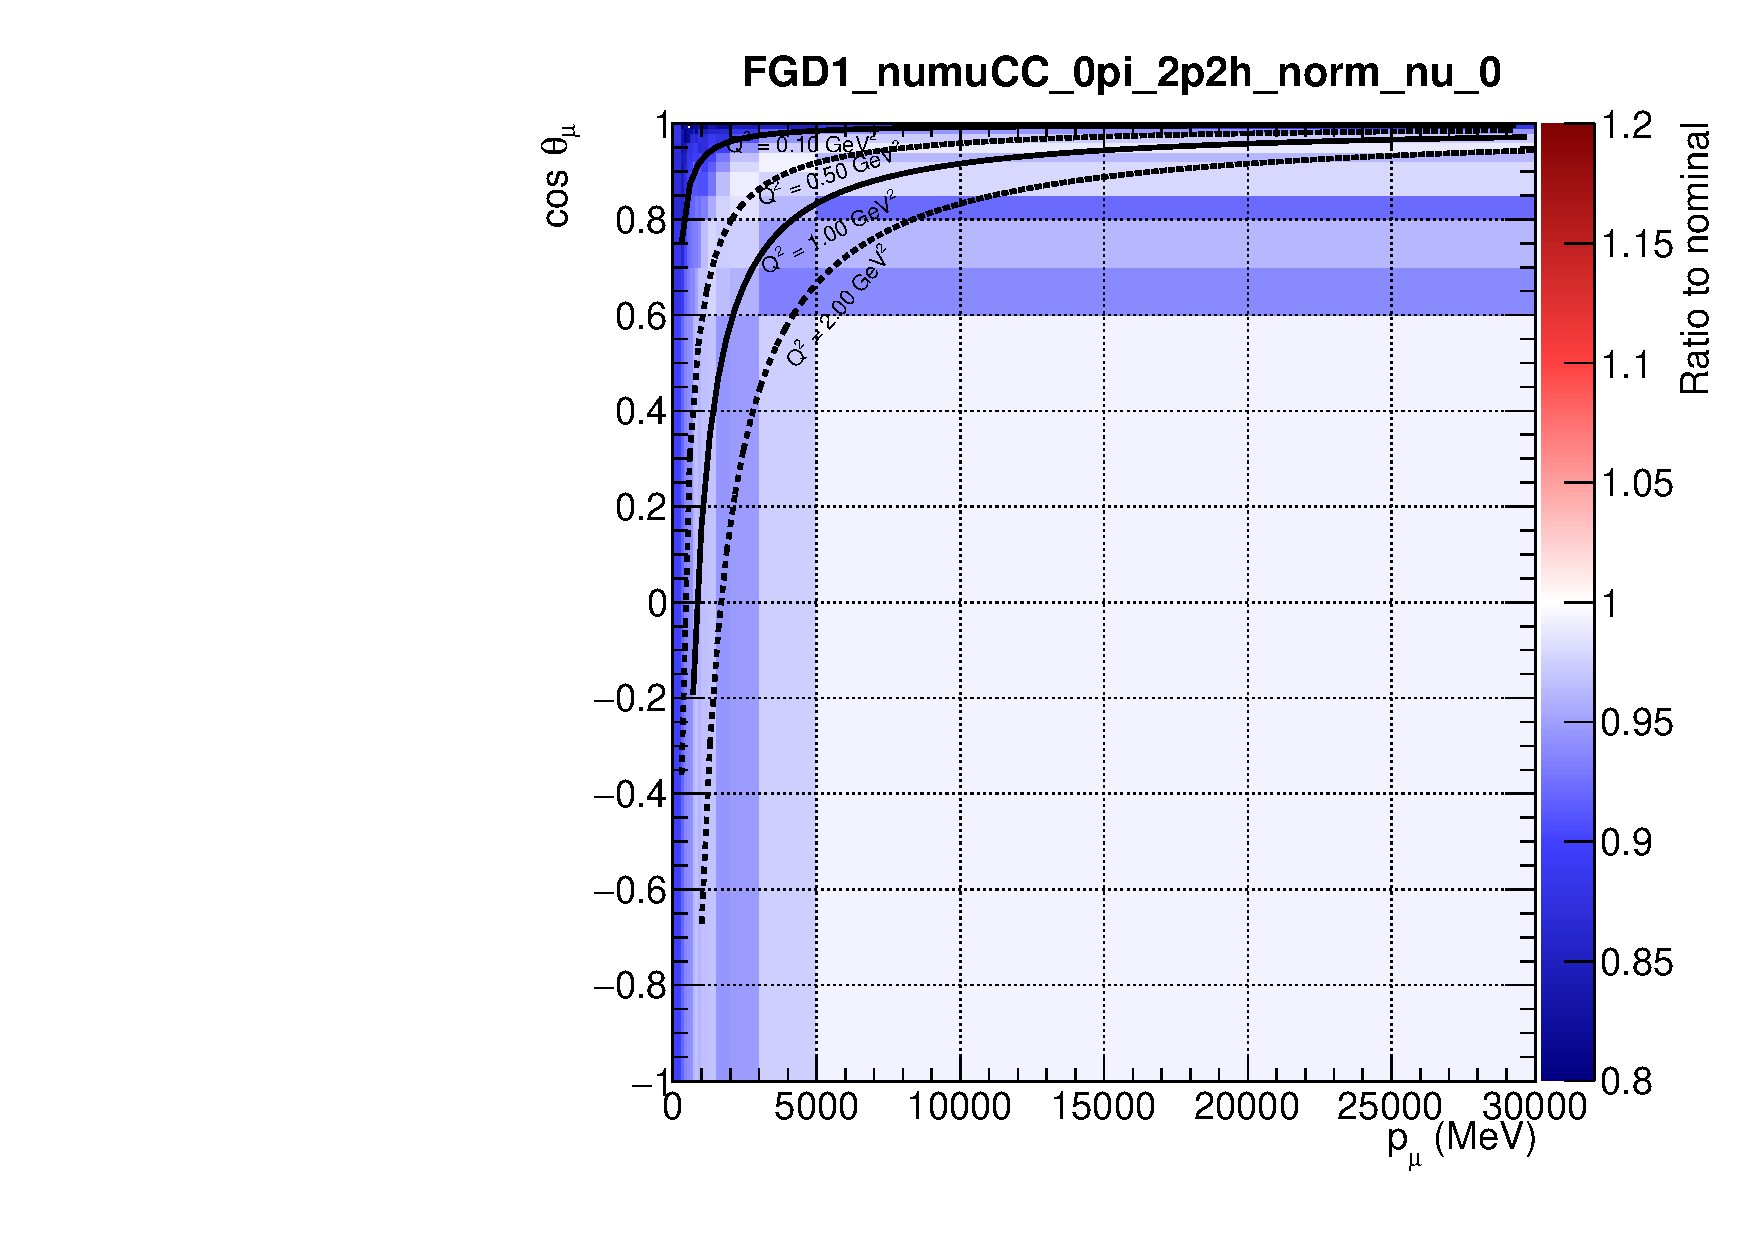
\includegraphics[width=\textwidth,page=1]{figures/mach3/sigmavar/Full_1sigmaVar_18July_BeRPA_U_ND280_sigmavar_highest_all}
	\end{subfigure}
	\begin{subfigure}[t]{0.24\textwidth}
	\includegraphics[width=\textwidth,page=2]{figures/mach3/sigmavar/Full_1sigmaVar_18July_BeRPA_U_ND280_sigmavar_highest_all}
	\end{subfigure}
	\begin{subfigure}[t]{0.24\textwidth}
	\includegraphics[width=\textwidth,page=3]{figures/mach3/sigmavar/Full_1sigmaVar_18July_BeRPA_U_ND280_sigmavar_highest_all}
	\end{subfigure}
	\begin{subfigure}[t]{0.24\textwidth}
	\includegraphics[width=\textwidth,page=4]{figures/mach3/sigmavar/Full_1sigmaVar_18July_BeRPA_U_ND280_sigmavar_highest_all}
	\end{subfigure}

	\begin{subfigure}[t]{0.24\textwidth}
	\includegraphics[width=\textwidth,page=7]{figures/mach3/sigmavar/Full_1sigmaVar_18July_BeRPA_U_ND280_sigmavar_highest_all}
	\end{subfigure}
	\begin{subfigure}[t]{0.24\textwidth}
	\includegraphics[width=\textwidth,page=8]{figures/mach3/sigmavar/Full_1sigmaVar_18July_BeRPA_U_ND280_sigmavar_highest_all}
	\end{subfigure}
	\begin{subfigure}[t]{0.24\textwidth}
		\includegraphics[width=\textwidth,page=9]{figures/mach3/sigmavar/Full_1sigmaVar_18July_BeRPA_U_ND280_sigmavar_highest_all}
	\end{subfigure}
	\begin{subfigure}[t]{0.24\textwidth}
		\includegraphics[width=\textwidth,page=10]{figures/mach3/sigmavar/Full_1sigmaVar_18July_BeRPA_U_ND280_sigmavar_highest_all}
	\end{subfigure}

\begin{subfigure}[t]{0.24\textwidth}
	\includegraphics[width=\textwidth,page=5]{figures/mach3/sigmavar/Full_1sigmaVar_18July_BeRPA_U_ND280_sigmavar_highest_all}
\end{subfigure}
\begin{subfigure}[t]{0.24\textwidth}
	\includegraphics[width=\textwidth,page=6]{figures/mach3/sigmavar/Full_1sigmaVar_18July_BeRPA_U_ND280_sigmavar_highest_all}
\end{subfigure}
\begin{subfigure}[t]{0.24\textwidth}
\includegraphics[width=\textwidth,page=11]{figures/mach3/sigmavar/Full_1sigmaVar_18July_BeRPA_U_ND280_sigmavar_highest_all}
\end{subfigure}
\begin{subfigure}[t]{0.24\textwidth}
\includegraphics[width=\textwidth,page=12]{figures/mach3/sigmavar/Full_1sigmaVar_18July_BeRPA_U_ND280_sigmavar_highest_all}
\end{subfigure}
\caption{The largest effect of the 1-$\sigma$ variations on FHC selections' \pmu \cosmu}
\label{fig:onesigma_fhc}
\end{figure}

\begin{figure}[h]
\begin{subfigure}[t]{0.24\textwidth}
	\includegraphics[width=\textwidth,page=13]{figures/mach3/sigmavar/Full_1sigmaVar_18July_BeRPA_U_ND280_sigmavar_highest_all}
\end{subfigure}
\begin{subfigure}[t]{0.24\textwidth}
	\includegraphics[width=\textwidth,page=14]{figures/mach3/sigmavar/Full_1sigmaVar_18July_BeRPA_U_ND280_sigmavar_highest_all}
	\end{subfigure}
\begin{subfigure}[t]{0.24\textwidth}
\includegraphics[width=\textwidth,page=15]{figures/mach3/sigmavar/Full_1sigmaVar_18July_BeRPA_U_ND280_sigmavar_highest_all}
\end{subfigure}
\begin{subfigure}[t]{0.24\textwidth}
\includegraphics[width=\textwidth,page=16]{figures/mach3/sigmavar/Full_1sigmaVar_18July_BeRPA_U_ND280_sigmavar_highest_all}
\end{subfigure}

\begin{subfigure}[t]{0.24\textwidth}
	\includegraphics[width=\textwidth,page=17]{figures/mach3/sigmavar/Full_1sigmaVar_18July_BeRPA_U_ND280_sigmavar_highest_all}
\end{subfigure}
\begin{subfigure}[t]{0.24\textwidth}
	\includegraphics[width=\textwidth,page=18]{figures/mach3/sigmavar/Full_1sigmaVar_18July_BeRPA_U_ND280_sigmavar_highest_all}
	\end{subfigure}
\begin{subfigure}[t]{0.24\textwidth}
\includegraphics[width=\textwidth,page=19]{figures/mach3/sigmavar/Full_1sigmaVar_18July_BeRPA_U_ND280_sigmavar_highest_all}
\end{subfigure}
\begin{subfigure}[t]{0.24\textwidth}
\includegraphics[width=\textwidth,page=20]{figures/mach3/sigmavar/Full_1sigmaVar_18July_BeRPA_U_ND280_sigmavar_highest_all}
\end{subfigure}

\begin{subfigure}[t]{0.24\textwidth}
	\includegraphics[width=\textwidth,page=21]{figures/mach3/sigmavar/Full_1sigmaVar_18July_BeRPA_U_ND280_sigmavar_highest_all}
\end{subfigure}
\begin{subfigure}[t]{0.24\textwidth}
	\includegraphics[width=\textwidth,page=22]{figures/mach3/sigmavar/Full_1sigmaVar_18July_BeRPA_U_ND280_sigmavar_highest_all}
\end{subfigure}
\begin{subfigure}[t]{0.24\textwidth}
\includegraphics[width=\textwidth,page=23]{figures/mach3/sigmavar/Full_1sigmaVar_18July_BeRPA_U_ND280_sigmavar_highest_all}
\end{subfigure}
\begin{subfigure}[t]{0.24\textwidth}
\includegraphics[width=\textwidth,page=24]{figures/mach3/sigmavar/Full_1sigmaVar_18July_BeRPA_U_ND280_sigmavar_highest_all}
\end{subfigure}

\begin{subfigure}[t]{0.24\textwidth}
	\includegraphics[width=\textwidth,page=25]{figures/mach3/sigmavar/Full_1sigmaVar_18July_BeRPA_U_ND280_sigmavar_highest_all}
\end{subfigure}
\begin{subfigure}[t]{0.24\textwidth}
	\includegraphics[width=\textwidth,page=26]{figures/mach3/sigmavar/Full_1sigmaVar_18July_BeRPA_U_ND280_sigmavar_highest_all}
\end{subfigure}
\begin{subfigure}[t]{0.24\textwidth}
	\includegraphics[width=\textwidth,page=27]{figures/mach3/sigmavar/Full_1sigmaVar_18July_BeRPA_U_ND280_sigmavar_highest_all}
\end{subfigure}
\begin{subfigure}[t]{0.24\textwidth}
	\includegraphics[width=\textwidth,page=28]{figures/mach3/sigmavar/Full_1sigmaVar_18July_BeRPA_U_ND280_sigmavar_highest_all}
\end{subfigure}

\caption{The largest effect of the 1-$\sigma$ variations on RHC selections' \pmu \cosmu}
\label{fig:onesigma_rhc}
\end{figure}

%beam+ND280+xsec
%Largest difference for FGD1_numuCC_0pi: 1584.73 (FGD1_numuCC_0pi_2p2h_norm_nu)
%Largest difference for FGD1_numuCC_1pi: 365.358 (FGD1_numuCC_1pi_CA5)
%Largest difference for FGD1_numuCC_other: 252.769 (FGD1_numuCC_other_CC_DIS)
%Largest difference for FGD2_numuCC_0pi: 1538.91 (FGD2_numuCC_0pi_2p2h_norm_nu)
%Largest difference for FGD2_numuCC_1pi: 288.216 (FGD2_numuCC_1pi_CA5)
%Largest difference for FGD2_numuCC_other: 227.53 (FGD2_numuCC_other_CC_DIS)
%Largest difference for FGD1_anti-numuCC_QE: 342.054 (FGD1_anti-numuCC_QE_2p2h_norm_nubar)
%Largest difference for FGD1_anti-numuCC_nQE: 59.3502 (FGD1_anti-numuCC_nQE_MARES)
%Largest difference for FGD2_anti-numuCC_1_track: 345.436 (FGD2_anti-numuCC_1_track_2p2h_norm_nubar)
%Largest difference for FGD2_anti-numuCC_N_tracks: 61.3828 (FGD2_anti-numuCC_N_tracks_MARES)
%Largest difference for FGD1_NuMuBkg_CCQE_in_AntiNu_Mode_: 93.3766 (FGD1_NuMuBkg_CCQE_in_AntiNu_Mode__2p2h_norm_nu)
%Largest difference for FGD1_NuMuBkg_CCnQE_in_AntiNu_Mode: 75.1545 (FGD1_NuMuBkg_CCnQE_in_AntiNu_Mode_b_29)
%Largest difference for FGD2_NuMuBkg_CCQE_in_AntiNu_Mode_: 92.3373 (FGD2_NuMuBkg_CCQE_in_AntiNu_Mode__2p2h_norm_nu)
%Largest difference for FGD2_NuMuBkg_CCnQE_in_AntiNu_Mode: 70.5455 (FGD2_NuMuBkg_CCnQE_in_AntiNu_Mode_MARES)

%beam+ND280
%Largest difference for FGD1_numuCC_0pi: 419.944 (FGD1_numuCC_0pi_b_4)
%Largest difference for FGD1_numuCC_1pi: 64.8746 (FGD1_numuCC_1pi_b_8)
%Largest difference for FGD1_numuCC_other: 104.927 (FGD1_numuCC_other_b_10)
%Largest difference for FGD2_numuCC_0pi: 428.013 (FGD2_numuCC_0pi_b_4)
%Largest difference for FGD2_numuCC_1pi: 54.6989 (FGD2_numuCC_1pi_b_8)
%Largest difference for FGD2_numuCC_other: 91.9717 (FGD2_numuCC_other_b_10)
%Largest difference for FGD1_anti-numuCC_QE: 95.0237 (FGD1_anti-numuCC_QE_b_34)
%Largest difference for FGD1_anti-numuCC_nQE: 29.915 (FGD1_anti-numuCC_nQE_b_29)
%Largest difference for FGD2_anti-numuCC_1_track: 95.1625 (FGD2_anti-numuCC_1_track_b_34)
%Largest difference for FGD2_anti-numuCC_N_tracks: 29.4032 (FGD2_anti-numuCC_N_tracks_b_29)
%Largest difference for FGD1_NuMuBkg_CCQE_in_AntiNu_Mode_: 37.1494 (FGD1_NuMuBkg_CCQE_in_AntiNu_Mode__b_29)
%Largest difference for FGD1_NuMuBkg_CCnQE_in_AntiNu_Mode: 75.1545 (FGD1_NuMuBkg_CCnQE_in_AntiNu_Mode_b_29)
%Largest difference for FGD2_NuMuBkg_CCQE_in_AntiNu_Mode_: 35.9022 (FGD2_NuMuBkg_CCQE_in_AntiNu_Mode__b_29)
%Largest difference for FGD2_NuMuBkg_CCnQE_in_AntiNu_Mode: 68.9212 (FGD2_NuMuBkg_CCnQE_in_AntiNu_Mode_b_29)

%ND280
%Largest difference for FGD1_numuCC_0pi: 306.549 (FGD1_numuCC_0pi_ndd_0)
%Largest difference for FGD1_numuCC_1pi: 31.2325 (FGD1_numuCC_1pi_ndd_50)
%Largest difference for FGD1_numuCC_other: 88.7887 (FGD1_numuCC_other_ndd_82)
%Largest difference for FGD2_numuCC_0pi: 354.861 (FGD2_numuCC_0pi_ndd_278)
%Largest difference for FGD2_numuCC_1pi: 31.2562 (FGD2_numuCC_1pi_ndd_328)
%Largest difference for FGD2_numuCC_other: 89.0011 (FGD2_numuCC_other_ndd_360)
%Largest difference for FGD1_anti-numuCC_QE: 43.0114 (FGD1_anti-numuCC_QE_ndd_133)
%Largest difference for FGD1_anti-numuCC_nQE: 12.409 (FGD1_anti-numuCC_nQE_ndd_183)
%Largest difference for FGD2_anti-numuCC_1_track: 46.6356 (FGD2_anti-numuCC_1_track_ndd_411)
%Largest difference for FGD2_anti-numuCC_N_tracks: 11.855 (FGD2_anti-numuCC_N_tracks_ndd_467)
%Largest difference for FGD1_NuMuBkg_CCQE_in_AntiNu_Mode_: 11.0608 (FGD1_NuMuBkg_CCQE_in_AntiNu_Mode__ndd_198)
%Largest difference for FGD1_NuMuBkg_CCnQE_in_AntiNu_Mode: 14.1052 (FGD1_NuMuBkg_CCnQE_in_AntiNu_Mode_ndd_239)
%Largest difference for FGD2_NuMuBkg_CCQE_in_AntiNu_Mode_: 10.5504 (FGD2_NuMuBkg_CCQE_in_AntiNu_Mode__ndd_476)
%Largest difference for FGD2_NuMuBkg_CCnQE_in_AntiNu_Mode: 15.3709 (FGD2_NuMuBkg_CCnQE_in_AntiNu_Mode_ndd_554)

\subsection{Prior Predictive Spectrum}
\label{sec:Asimov_prior}
The first statistical test on the Asimov is to investigate the prior predictive spectrum and resulting p-values. This is meant to reflect the compatibility of the prior with the Asimov data. The p-value is expected to be $\sim50\%$ since the parameter throws are either side of the central value which created the Asimov data set. However, the throws are correlated, so offsets from 50\% is to be expected. The two p-values are shown in \autoref{fig:prior_predictive_asimov} and lay around the expected value of 50\% as previously asserted.
\begin{figure}[h]
	\begin{subfigure}[t]{0.49\textwidth}
		\includegraphics[width=\textwidth, trim={0mm 0mm 0mm 11mm}, clip,page=1]{figures/mach3/Asimov/2017b_NewDet_3Xsec_4Det_5Flux_NewXSecTune_Asimov_merge_PriorPred_procs}
	\end{subfigure}
	\begin{subfigure}[t]{0.49\textwidth}
		\includegraphics[width=\textwidth, trim={0mm 0mm 0mm 11mm}, clip,page=2]{figures/mach3/Asimov/2017b_NewDet_3Xsec_4Det_5Flux_NewXSecTune_Asimov_merge_PriorPred_procs}
	\end{subfigure}
\caption{Prior predictive p-values for the Asimov data}
\label{fig:prior_predictive_asimov}
\end{figure}

\autoref{tab:asimov_prior_pred} shows the prior predictive event rates from the prior predictive spectrum to the Asmiov data with uncertainties from all systematics. Using the prior covariances without any fitting to the Asimov data produces 11\% uncertainty on the total event rate, with 13\% on the CC0$\pi$, 11\% on CC1$\pi$ and 13\% on CCOther. There is a particularly bad likelihood for the 0$\pi$ and 1Trk selections for the Asimov prior predictive spectrum. This is likely due to missing correlations between cross-section, flux and near-detector parameters, causing the correlated throws of the systematics to be skewed.
\begin{table}[h]
	\centering
	\begin{tabular}{l | c c | c}
		\hline
		\hline
		Sample & Nominal & Prior Pred & -2$\log\mathcal{L}_s$ \\ 
		\hline
		FGD1 0$\pi$ & 16723.8 &  $17014.5\pm2244.0$ &  14.58 \\
		FGD1 1$\pi$ & 4381.47 &  $4438.3\pm487.6$ &  0.99 \\
		FGD1 Other & 3943.95 &  $3984.1\pm537.5$  & 0.76\\
		
		FGD2 0$\pi$ & 16959.3 &  $17252.4\pm2311.7$ &  18.9 \\
		FGD2 1$\pi$ & 3564.23 &  $3612.9\pm398.4$ &  0.92 \\
		FGD2 Other & 3570.94 &  $3581.5\pm456.3$ &  0.92 \\
		\hline
		FGD1 1Trk & 3587.77 &  $3695.7\pm481.8$ &  3.99 \\
		FGD1 NTrk & 1066.91 &  $1093.9\pm138.4$ &  1.51  \\
		FGD2 1Trk & 3618.29 &  $3721.1\pm473.6$ &  3.89 \\
		FGD2 NTrk & 1077.24 &  $1102.9\pm131.6$ &  0.90 \\
		\hline
		FGD1 \numu 1 Trk & 1272.17 &  $1309.4\pm139.6$ &  1.27 \\
		FGD1 \numu NTrk & 1357.45 &  $1378.0\pm155.9$ &  0.50 \\
		FGD2 \numu 1Trk & 1262.63 &  $1305.9\pm140.9$ &  2.09 \\
		FGD2 \numu NTrk & 1246.71 &  $1263.5\pm139.4$ &  0.49 \\
		\hline
		Total & 63632.86 & $64670.8\pm7025.2$ & 51.72 \\
		\hline
		\hline
	\end{tabular}
	\caption{Event rates broken down by sample after the prior predictive spectrum for the Asimov data}
	\label{tab:asimov_prior_pred}
\end{table}

\subsection{Fitting to Asimov Data}
\label{sec:asimov_fit}
The model is here fit to the Asimov data set, defined as the model set to the central values of the prior constraints. Three different MCMCs are presented, each one being a tuned version of the previous, in regards to the autocorrelations and acceptance probability of each chain. \autoref{tab:asimov_mcmc_versions} shows the chains for the Asimov study. In each case the burn-in is 1/4 of the total chain length.
\begin{table}[h]
	\centering
	\begin{tabular}{l | c c c}
		\hline
		\hline
							& Chain length  & Acceptance rate & Accepted steps\\
							\hline
		Low acceptance		& 800,000		& 6.9\% 		  & 55,200 \\
		Mid acceptance		& 800,000		& 15.0\% 		  & 120,000\\
		High acceptance		& 1,400,000		& 23.0\%  		  & 322,000 \\
		\hline
		\hline
	\end{tabular}
\caption{Different MCMC run configurations for the Asimov fit}
\label{tab:asimov_mcmc_versions}
\end{table}

As covered in \autoref{chap:mcmc}, MCMC methods aren't designed to find a global minimum of the test-statistic, so we revert to defining the ``best-fit'' parameter set as the marginal posterior over all parameters except the ``parameter of interest''. Since we're marginalising over $\sim700$ parameters, the study is likely to see parameter ``biases'' from marginalisation effects.

\autoref{fig:mcmc_asimov_loglsteps} demonstrates that the lowest test-statistic is obtained right at the very beginning of the chain, which progresses to move around the minimum, scanning parameter combinations with $\chi^2 \sim 300-400$, here defined as $\chi^2 = -\log\mathcal{L}$, so $-2\log\mathcal{L}$ roughly coincides with the number of parameters in the fit. The lowest test-statistic after the burn-in is found at step 423471/800000, which has $\chi^2 = 284.49$.
\begin{figure}[h]
	\includegraphics[width=0.45\textwidth]{figures/mach3/mcmc/2017b_NewDet_3Xsec_4Det_5Flux_NewXSecTune_Asimov_merge}
	\caption{Markov Chain behaviour for the ``mid acceptance'' MCMC, showing intended behaviour of moving around minimum}
	\label{fig:mcmc_asimov_loglsteps}
\end{figure}

\autoref{fig:flux_asimov_fhc} (FHC) and \autoref{fig:flux_asimov_rhc} (RHC) shows the result of the Asimov fit for the ND280 flux parameters. There is a consistent ``bias'' in estimating the parameter set which generated the Asimov, whose residuals (bottom panel) appear to have a shape, going from over-estimated to under-estimated as $E_\nu$ increases. The highest acceptance chain has less ``bias'' than the shorter chains, and all the chains are consistent with each other. Many of the parameters with large biases are barely constrained by the ND280 data (e.g. ND280 FHC $\nu_\mu$ at $E_\nu > 4\text{ GeV}$ and ND280 RHC $\bar{\nu}_e$) and only get their constraints from the prior covariance matrix. The ND280 to SK correlation is working as expected and the SK flux parameters show almost identical constraint to their ND280 equivalents.

We note improved constraints on all flux parameters from the prior uncertainty. This is strongest around the flux peak at $E_\nu \sim 0.6\text{ GeV}$, where the flux parameter uncertainty reduces by 50\%.
\begin{figure}[h]
	\begin{subfigure}[t]{0.24\textwidth}
		\includegraphics[width=\textwidth, trim={0mm 150mm 50mm 0mm}, clip,page=1]{figures/mach3/Asimov/2017_NewDet_Asimov_actually_0_2017b_NewDet_3Xsec_4Det_5Flux_NewXSecTune_Asimov_0_2017b_NewDet_NewData_Asimov_Long_0}
	\end{subfigure}
\begin{subfigure}[t]{0.24\textwidth}
\includegraphics[width=\textwidth, trim={0mm 100mm 50mm 50mm}, clip,page=1]{figures/mach3/Asimov/2017_NewDet_Asimov_actually_0_2017b_NewDet_3Xsec_4Det_5Flux_NewXSecTune_Asimov_0_2017b_NewDet_NewData_Asimov_Long_0}
\end{subfigure}
\begin{subfigure}[t]{0.24\textwidth}
\includegraphics[width=\textwidth, trim={0mm 50mm 50mm 100mm}, clip,page=1]{figures/mach3/Asimov/2017_NewDet_Asimov_actually_0_2017b_NewDet_3Xsec_4Det_5Flux_NewXSecTune_Asimov_0_2017b_NewDet_NewData_Asimov_Long_0}
\end{subfigure}
\begin{subfigure}[t]{0.24\textwidth}
\includegraphics[width=\textwidth, trim={0mm 0mm 50mm 150mm}, clip,page=1]{figures/mach3/Asimov/2017_NewDet_Asimov_actually_0_2017b_NewDet_3Xsec_4Det_5Flux_NewXSecTune_Asimov_0_2017b_NewDet_NewData_Asimov_Long_0}
\end{subfigure}

\begin{subfigure}[t]{0.24\textwidth}
	\includegraphics[width=\textwidth, trim={0mm 0mm 0mm 0mm}, clip,page=2]{figures/mach3/Asimov/2017_NewDet_Asimov_actually_0_2017b_NewDet_3Xsec_4Det_5Flux_NewXSecTune_Asimov_0_2017b_NewDet_NewData_Asimov_Long_0}
\end{subfigure}
\begin{subfigure}[t]{0.24\textwidth}
	\includegraphics[width=\textwidth, trim={0mm 0mm 0mm 0mm}, clip,page=3]{figures/mach3/Asimov/2017_NewDet_Asimov_actually_0_2017b_NewDet_3Xsec_4Det_5Flux_NewXSecTune_Asimov_0_2017b_NewDet_NewData_Asimov_Long_0}
\end{subfigure}
\begin{subfigure}[t]{0.24\textwidth}
	\includegraphics[width=\textwidth, trim={0mm 0mm 0mm 0mm}, clip,page=4]{figures/mach3/Asimov/2017_NewDet_Asimov_actually_0_2017b_NewDet_3Xsec_4Det_5Flux_NewXSecTune_Asimov_0_2017b_NewDet_NewData_Asimov_Long_0}
\end{subfigure}
\begin{subfigure}[t]{0.24\textwidth}
	\includegraphics[width=\textwidth, trim={0mm 0mm 0mm 0mm}, clip,page=5]{figures/mach3/Asimov/2017_NewDet_Asimov_actually_0_2017b_NewDet_3Xsec_4Det_5Flux_NewXSecTune_Asimov_0_2017b_NewDet_NewData_Asimov_Long_0}
\end{subfigure}

\begin{subfigure}[t]{0.24\textwidth}
	\includegraphics[width=\textwidth, trim={0mm 0mm 0mm 0mm}, clip,page=10]{figures/mach3/Asimov/2017_NewDet_Asimov_actually_0_2017b_NewDet_3Xsec_4Det_5Flux_NewXSecTune_Asimov_0_2017b_NewDet_NewData_Asimov_Long_0}
\end{subfigure}
\begin{subfigure}[t]{0.24\textwidth}
	\includegraphics[width=\textwidth, trim={0mm 0mm 0mm 0mm}, clip,page=11]{figures/mach3/Asimov/2017_NewDet_Asimov_actually_0_2017b_NewDet_3Xsec_4Det_5Flux_NewXSecTune_Asimov_0_2017b_NewDet_NewData_Asimov_Long_0}
\end{subfigure}
\begin{subfigure}[t]{0.24\textwidth}
	\includegraphics[width=\textwidth, trim={0mm 0mm 0mm 0mm}, clip,page=12]{figures/mach3/Asimov/2017_NewDet_Asimov_actually_0_2017b_NewDet_3Xsec_4Det_5Flux_NewXSecTune_Asimov_0_2017b_NewDet_NewData_Asimov_Long_0}
\end{subfigure}
\begin{subfigure}[t]{0.24\textwidth}
	\includegraphics[width=\textwidth, trim={0mm 0mm 0mm 0mm}, clip,page=13]{figures/mach3/Asimov/2017_NewDet_Asimov_actually_0_2017b_NewDet_3Xsec_4Det_5Flux_NewXSecTune_Asimov_0_2017b_NewDet_NewData_Asimov_Long_0}
\end{subfigure}
\caption{ND280 and SK FHC flux parameters after the Asimov fit for different MCMC chains}
\label{fig:flux_asimov_fhc}
\end{figure}

\begin{figure}[h]
	\begin{subfigure}[t]{0.24\textwidth}
		\includegraphics[width=\textwidth, trim={0mm 150mm 50mm 0mm}, clip,page=1]{figures/mach3/Asimov/2017_NewDet_Asimov_actually_0_2017b_NewDet_3Xsec_4Det_5Flux_NewXSecTune_Asimov_0_2017b_NewDet_NewData_Asimov_Long_0}
	\end{subfigure}
	\begin{subfigure}[t]{0.24\textwidth}
		\includegraphics[width=\textwidth, trim={0mm 100mm 50mm 50mm}, clip,page=1]{figures/mach3/Asimov/2017_NewDet_Asimov_actually_0_2017b_NewDet_3Xsec_4Det_5Flux_NewXSecTune_Asimov_0_2017b_NewDet_NewData_Asimov_Long_0}
	\end{subfigure}
	\begin{subfigure}[t]{0.24\textwidth}
		\includegraphics[width=\textwidth, trim={0mm 50mm 50mm 100mm}, clip,page=1]{figures/mach3/Asimov/2017_NewDet_Asimov_actually_0_2017b_NewDet_3Xsec_4Det_5Flux_NewXSecTune_Asimov_0_2017b_NewDet_NewData_Asimov_Long_0}
	\end{subfigure}
	\begin{subfigure}[t]{0.24\textwidth}
		\includegraphics[width=\textwidth, trim={0mm 0mm 50mm 150mm}, clip,page=1]{figures/mach3/Asimov/2017_NewDet_Asimov_actually_0_2017b_NewDet_3Xsec_4Det_5Flux_NewXSecTune_Asimov_0_2017b_NewDet_NewData_Asimov_Long_0}
	\end{subfigure}

	\begin{subfigure}[t]{0.24\textwidth}
		\includegraphics[width=\textwidth, trim={0mm 0mm 0mm 0mm}, clip,page=6]{figures/mach3/Asimov/2017_NewDet_Asimov_actually_0_2017b_NewDet_3Xsec_4Det_5Flux_NewXSecTune_Asimov_0_2017b_NewDet_NewData_Asimov_Long_0}
	\end{subfigure}
	\begin{subfigure}[t]{0.24\textwidth}
		\includegraphics[width=\textwidth, trim={0mm 0mm 0mm 0mm}, clip,page=7]{figures/mach3/Asimov/2017_NewDet_Asimov_actually_0_2017b_NewDet_3Xsec_4Det_5Flux_NewXSecTune_Asimov_0_2017b_NewDet_NewData_Asimov_Long_0}
	\end{subfigure}
	\begin{subfigure}[t]{0.24\textwidth}
		\includegraphics[width=\textwidth, trim={0mm 0mm 0mm 0mm}, clip,page=8]{figures/mach3/Asimov/2017_NewDet_Asimov_actually_0_2017b_NewDet_3Xsec_4Det_5Flux_NewXSecTune_Asimov_0_2017b_NewDet_NewData_Asimov_Long_0}
	\end{subfigure}
	\begin{subfigure}[t]{0.24\textwidth}
		\includegraphics[width=\textwidth, trim={0mm 0mm 0mm 0mm}, clip,page=9]{figures/mach3/Asimov/2017_NewDet_Asimov_actually_0_2017b_NewDet_3Xsec_4Det_5Flux_NewXSecTune_Asimov_0_2017b_NewDet_NewData_Asimov_Long_0}
		\end{subfigure}
		
	\begin{subfigure}[t]{0.24\textwidth}
		\includegraphics[width=\textwidth, trim={0mm 0mm 0mm 0mm}, clip,page=14]{figures/mach3/Asimov/2017_NewDet_Asimov_actually_0_2017b_NewDet_3Xsec_4Det_5Flux_NewXSecTune_Asimov_0_2017b_NewDet_NewData_Asimov_Long_0}
	\end{subfigure}
	\begin{subfigure}[t]{0.24\textwidth}
		\includegraphics[width=\textwidth, trim={0mm 0mm 0mm 0mm}, clip,page=15]{figures/mach3/Asimov/2017_NewDet_Asimov_actually_0_2017b_NewDet_3Xsec_4Det_5Flux_NewXSecTune_Asimov_0_2017b_NewDet_NewData_Asimov_Long_0}
	\end{subfigure}
	\begin{subfigure}[t]{0.24\textwidth}
		\includegraphics[width=\textwidth, trim={0mm 0mm 0mm 0mm}, clip,page=16]{figures/mach3/Asimov/2017_NewDet_Asimov_actually_0_2017b_NewDet_3Xsec_4Det_5Flux_NewXSecTune_Asimov_0_2017b_NewDet_NewData_Asimov_Long_0}
	\end{subfigure}
	\begin{subfigure}[t]{0.24\textwidth}
		\includegraphics[width=\textwidth, trim={0mm 0mm 0mm 0mm}, clip,page=17]{figures/mach3/Asimov/2017_NewDet_Asimov_actually_0_2017b_NewDet_3Xsec_4Det_5Flux_NewXSecTune_Asimov_0_2017b_NewDet_NewData_Asimov_Long_0}
	\end{subfigure}
	\caption{ND280 and SK RHC flux parameters after the Asimov fit for different MCMC chains}
	\label{fig:flux_asimov_rhc}
\end{figure}

\autoref{fig:xsec_asimov} shows interaction parameters after the fit to Asimov data. As for the flux parameters, some parameters are ``biased'', notably the Fermi momentum parameters ($p_F$), 2p2h norm $\bar{\nu}$, BeRPA A, CC DIS and NC$1\gamma$. Again, the chains are very compatible in their estimates of the parameter values, and the reduction of the uncertainties are significant for many parameters. $p_F$, 2p2h norm C/O, BeRPA E, $\nu_e$/$\nu_\mu$, NC coherent, NC$1\gamma$ and NC oth. SK barely improve due to the fit lacking events which constrain these parameters, and/or the parameter has very little ``strength'' to change the interaction cross-section.
\begin{figure}[h]
	\begin{subfigure}[t]{0.24\textwidth}
		\includegraphics[width=\textwidth, trim={0mm 150mm 50mm 0mm}, clip,page=1]{figures/mach3/Asimov/2017_NewDet_Asimov_actually_0_2017b_NewDet_3Xsec_4Det_5Flux_NewXSecTune_Asimov_0_2017b_NewDet_NewData_Asimov_Long_0}
	\end{subfigure}
	\begin{subfigure}[t]{0.24\textwidth}
		\includegraphics[width=\textwidth, trim={0mm 100mm 50mm 50mm}, clip,page=1]{figures/mach3/Asimov/2017_NewDet_Asimov_actually_0_2017b_NewDet_3Xsec_4Det_5Flux_NewXSecTune_Asimov_0_2017b_NewDet_NewData_Asimov_Long_0}
	\end{subfigure}
	\begin{subfigure}[t]{0.24\textwidth}
		\includegraphics[width=\textwidth, trim={0mm 50mm 50mm 100mm}, clip,page=1]{figures/mach3/Asimov/2017_NewDet_Asimov_actually_0_2017b_NewDet_3Xsec_4Det_5Flux_NewXSecTune_Asimov_0_2017b_NewDet_NewData_Asimov_Long_0}
	\end{subfigure}
	\begin{subfigure}[t]{0.24\textwidth}
		\includegraphics[width=\textwidth, trim={0mm 0mm 50mm 150mm}, clip,page=1]{figures/mach3/Asimov/2017_NewDet_Asimov_actually_0_2017b_NewDet_3Xsec_4Det_5Flux_NewXSecTune_Asimov_0_2017b_NewDet_NewData_Asimov_Long_0}
	\end{subfigure}

	\begin{subfigure}[t]{0.49\textwidth}
		\includegraphics[width=\textwidth, trim={0mm 0mm 0mm 0mm}, clip,page=18]{figures/mach3/Asimov/2017_NewDet_Asimov_actually_0_2017b_NewDet_3Xsec_4Det_5Flux_NewXSecTune_Asimov_0_2017b_NewDet_NewData_Asimov_Long_0}
	\end{subfigure}
	\begin{subfigure}[t]{0.49\textwidth}
		\includegraphics[width=\textwidth, trim={0mm 0mm 0mm 0mm}, clip,page=19]{figures/mach3/Asimov/2017_NewDet_Asimov_actually_0_2017b_NewDet_3Xsec_4Det_5Flux_NewXSecTune_Asimov_0_2017b_NewDet_NewData_Asimov_Long_0}
	\end{subfigure}

	\begin{subfigure}[t]{0.49\textwidth}
		\includegraphics[width=\textwidth, trim={0mm 0mm 0mm 0mm}, clip,page=20]{figures/mach3/Asimov/2017_NewDet_Asimov_actually_0_2017b_NewDet_3Xsec_4Det_5Flux_NewXSecTune_Asimov_0_2017b_NewDet_NewData_Asimov_Long_0}
	\end{subfigure}
	\begin{subfigure}[t]{0.49\textwidth}
		\includegraphics[width=\textwidth, trim={0mm 0mm 0mm 0mm}, clip,page=21]{figures/mach3/Asimov/2017_NewDet_Asimov_actually_0_2017b_NewDet_3Xsec_4Det_5Flux_NewXSecTune_Asimov_0_2017b_NewDet_NewData_Asimov_Long_0}
	\end{subfigure}
	\caption{Interaction parameters after the Asimov fit for different MCMC chains}
	\label{fig:xsec_asimov}
\end{figure}

\subsubsection{Fitting to Asimov Data, Varying Only Flux Parameters}
To investigate if correlations and marginalisation are to blame for the ``bias'' in \autoref{sec:asimov_fit}, a fit to the Asimov data is done keeping the cross-section and ND280 parameters fixed at their Asimov values, and only the flux parameters are varied. \autoref{fig:flux_asimov_nd280_fluxonly} shows the parameter values for the ND280 flux parameters using different methods of obtaining the central values. The biases have vanished for all methods, and we conclude that the Asimov parameters are being correctly found when flux parameters alone are being fit.

\begin{figure}[h]
	\begin{subfigure}[t]{0.24\textwidth}
		\includegraphics[width=\textwidth, trim={0mm 150mm 30mm 0mm}, clip,page=1]{figures/mach3/Asimov/2017b_Asimov_July2017_FixND280_FixXsec_0_drawPar}
	\end{subfigure}
\begin{subfigure}[t]{0.24\textwidth}
	\includegraphics[width=\textwidth, trim={0mm 100mm 30mm 50mm}, clip,page=1]{figures/mach3/Asimov/2017b_Asimov_July2017_FixND280_FixXsec_0_drawPar}
\end{subfigure}
\begin{subfigure}[t]{0.24\textwidth}
	\includegraphics[width=\textwidth, trim={0mm 50mm 30mm 100mm}, clip,page=1]{figures/mach3/Asimov/2017b_Asimov_July2017_FixND280_FixXsec_0_drawPar}
\end{subfigure}
\begin{subfigure}[t]{0.24\textwidth}
	\includegraphics[width=\textwidth, trim={0mm 0mm 30mm 150mm}, clip,page=1]{figures/mach3/Asimov/2017b_Asimov_July2017_FixND280_FixXsec_0_drawPar}
\end{subfigure}
	
	\begin{subfigure}[t]{0.24\textwidth}
		\includegraphics[width=\textwidth, trim={0mm 0mm 0mm 0mm}, clip,page=2]{figures/mach3/Asimov/2017b_Asimov_July2017_FixND280_FixXsec_0_drawPar}
	\end{subfigure}
	\begin{subfigure}[t]{0.24\textwidth}
		\includegraphics[width=\textwidth, trim={0mm 0mm 0mm 0mm}, clip,page=3]{figures/mach3/Asimov/2017b_Asimov_July2017_FixND280_FixXsec_0_drawPar}
	\end{subfigure}
	\begin{subfigure}[t]{0.24\textwidth}
		\includegraphics[width=\textwidth, trim={0mm 0mm 0mm 0mm}, clip,page=4]{figures/mach3/Asimov/2017b_Asimov_July2017_FixND280_FixXsec_0_drawPar}
	\end{subfigure}
	\begin{subfigure}[t]{0.24\textwidth}
		\includegraphics[width=\textwidth, trim={0mm 0mm 0mm 0mm}, clip,page=5]{figures/mach3/Asimov/2017b_Asimov_July2017_FixND280_FixXsec_0_drawPar}
	\end{subfigure}
	
	\begin{subfigure}[t]{0.24\textwidth}
		\includegraphics[width=\textwidth, trim={0mm 0mm 0mm 0mm}, clip,page=6]{figures/mach3/Asimov/2017b_Asimov_July2017_FixND280_FixXsec_0_drawPar}
	\end{subfigure}
	\begin{subfigure}[t]{0.24\textwidth}
		\includegraphics[width=\textwidth, trim={0mm 0mm 0mm 0mm}, clip,page=7]{figures/mach3/Asimov/2017b_Asimov_July2017_FixND280_FixXsec_0_drawPar}
	\end{subfigure}
	\begin{subfigure}[t]{0.24\textwidth}
		\includegraphics[width=\textwidth, trim={0mm 0mm 0mm 0mm}, clip,page=8]{figures/mach3/Asimov/2017b_Asimov_July2017_FixND280_FixXsec_0_drawPar}
	\end{subfigure}
	\begin{subfigure}[t]{0.24\textwidth}
		\includegraphics[width=\textwidth, trim={0mm 0mm 0mm 0mm}, clip,page=9]{figures/mach3/Asimov/2017b_Asimov_July2017_FixND280_FixXsec_0_drawPar}
	\end{subfigure}
	
	\caption{ND280 flux parameters after the Asimov fit, fitting flux only}
	\label{fig:flux_asimov_nd280_fluxonly}
\end{figure}

\subsubsection{Marginalisation Effects}
\label{sec:marginalisation}
Marginalisation effects are expected for parameters which correlate strongly with non-Gaussian parameters, which are present in this analysis. This is investigated further by looking at the two-dimensional marginal posteriors for a few correlated parameters and comparing them to their one-dimensional marginal posterior. For the central value parameter estimates we use the highest posterior density point. We look at three selected parameters that show bias: $p_F^{C}$, 2p2h norm $\bar{\nu}$ and the 30th beam parameter (``$b_{29}$'', which is the ND280 RHC $\bar{\nu}_\mu$ parameter for $E_\nu= 0.7-1.0\text{ GeV}$).

\paragraph{$p_F^C$ bias}
\autoref{fig:marginalisation_pf} shows the two dimensional marginal posterior of $p_F^C$ with $p_F^O$ and BeRPA D. The $p_F$ parameters are problematic in that the parameterisation allows for non-Gaussian behaviour and additionally has hard cut-offs near the prior value--notably at the lower limit. Marginalising over such parameters causes shifts in the localtion of the highest posterior density. For the two-dimensional posterior of $p_F^C$ and $p_F^O$ the highest density is very close to the prior input value of 1.0 for both parameters (within one bin-width), whereas marginalising over the other parameter causes the posterior density to shift from $p_F^{C}$ = 1.008 to 1.062. The second inset shows the opposite effect when marginalising $p_F^{C}$ over BeRPA D, in which the two-dimensional marginal posterior has its highest density at $p_F^{C} = 1.077$ which shifts to $p_F^{C} = 1.054$ after the marginalisation.
\begin{figure}[h]
	\begin{subfigure}[t]{0.49\textwidth}
		\includegraphics[width=\textwidth, trim={0mm 0mm 0mm 0mm}, clip,page=15]{figures/mach3/mcmc/2017b_NewDet_3Xsec_4Det_5Flux_NewXSecTune_Asimov_merge_marg_xsec}
	\end{subfigure}
	\begin{subfigure}[t]{0.49\textwidth}
		\includegraphics[width=\textwidth, trim={0mm 0mm 0mm 0mm}, clip,page=23]{figures/mach3/mcmc/2017b_NewDet_3Xsec_4Det_5Flux_NewXSecTune_Asimov_merge_marg_xsec}
	\end{subfigure}
\caption{Selected two-dimensional marginal posteriors for $p_F^C$ and 2p2h shape O and BeRPA B, showing the resulting one-dimensional marginal posterior}
\label{fig:marginalisation_pf}
\end{figure}

\paragraph{2p2h norm $\bar{\nu}_\mu$ bias}
\autoref{fig:marginalisation_2p2h_norm_nubar} shows the same marginalisation plots for 2p2h norm $\bar{\nu}$ with 2p2h shape C and BeRPA E. The case of the 2p2h normalisation parameters is slightly different to the $p_F$ parameters: the normalisation is well-behaved across the phase space, looks Gaussian, and does not have any hard cut-offs near the prior\footnote{The cut-off is when the normalisation reaches 0}. The marginsaliation effect instead happens with parameters that 2p2h normalisations correlate with, which may have non-Gaussian posterior shapes. The first example is with 2p2h shape C, in which we notice a tail at low 2p2h shape C and low 2p2h norm $\bar{\nu}$. Marginalising over the parameter brings the posterior density from 2p2h norm $\bar{\nu}$ = 1.061 to 0.842, which is the main cause of the ``bias''. Again, other parameters have the opposite effect: marginalising over BeRPA E causes the marginal posterior to shift from 2p2h norm $\bar{\nu}$ from 0.769 to 0.842.
\begin{figure}[h]
	\begin{subfigure}[t]{0.49\textwidth}
		\includegraphics[width=\textwidth, trim={0mm 0mm 0mm 0mm}, clip,page=55]{figures/mach3/mcmc/2017b_NewDet_3Xsec_4Det_5Flux_NewXSecTune_Asimov_merge_marg_xsec}
	\end{subfigure}
	\begin{subfigure}[t]{0.49\textwidth}
		\includegraphics[width=\textwidth, trim={0mm 0mm 0mm 0mm}, clip,page=60]{figures/mach3/mcmc/2017b_NewDet_3Xsec_4Det_5Flux_NewXSecTune_Asimov_merge_marg_xsec}
	\end{subfigure}
	\caption{Selected two-dimensional marginal posteriors for 2p2h norm $\bar{\nu}$ with 2p2h shape C and BeRPA E showing the resulting one-dimensional marginal posterior}
	\label{fig:marginalisation_2p2h_norm_nubar}
\end{figure}

\paragraph{$b\_29$ bias}
The 30th beam parameter (``$b\_29$'', the ND280 RHC $\bar{\nu}_\mu$ parameter for $E_\nu= 0.7-1.0\text{ GeV}$) sees similar effects from a number of parameters: ``$b\_24$'' (ND280 FHC $\bar{\nu}_e$ 2.5-30 GeV), ``$b\_46$'' (ND280 RHC $\nu_\mu$ 1.5-2.5 GeV), ``$b\_49$'' (ND280 RHC $\nu_e$ 2.5-30 GeV) and BeRPA D. The marginalisation plots are shown in \autoref{fig:marginalisation_b29} and all the above parameters have identical shifts: $b\_29$ moves from 0.988 to 0.974. It is noteworthy that the above parameters are all only weakly constrained by ND280 data: there is no dedicated $\nu_e$ selection (b\_46 and b\_49 control $\nu_e$ flux) and high $Q^2$ CCQE events are sparse (the region for BeRPA D). This can cause non-Gaussianity in that the chain may ``wander'' the space and explore a largely flat likelihood in parameters.
\begin{figure}[h]
	\begin{subfigure}[t]{0.24\textwidth}
		\includegraphics[width=\textwidth, trim={0mm 0mm 0mm 0mm}, clip,page=25]{figures/mach3/mcmc/2017b_NewDet_3Xsec_4Det_5Flux_NewXSecTune_Asimov_merge_b29}
	\end{subfigure}
	\begin{subfigure}[t]{0.24\textwidth}
		\includegraphics[width=\textwidth, trim={0mm 0mm 0mm 0mm}, clip,page=47]{figures/mach3/mcmc/2017b_NewDet_3Xsec_4Det_5Flux_NewXSecTune_Asimov_merge_b29}
	\end{subfigure}
	\begin{subfigure}[t]{0.24\textwidth}
		\includegraphics[width=\textwidth, trim={0mm 0mm 0mm 0mm}, clip,page=50]{figures/mach3/mcmc/2017b_NewDet_3Xsec_4Det_5Flux_NewXSecTune_Asimov_merge_b29}
	\end{subfigure}
	\begin{subfigure}[t]{0.24\textwidth}
		\includegraphics[width=\textwidth, trim={0mm 0mm 0mm 0mm}, clip,page=61]{figures/mach3/mcmc/2017b_NewDet_3Xsec_4Det_5Flux_NewXSecTune_Asimov_merge_b29}
	\end{subfigure}
	\caption{Selected two-dimensional marginal posteriors for ``$b\_29$'' (ND280 RHC $\bar{\nu}_\mu$ 0.7-1.0 GeV)}
	\label{fig:marginalisation_b29}
\end{figure}

In conclusion, the biases present in the Asmiov fit study seems likely to be due to marginlisation effects over parameters that are non-Gaussian, have hard cut-offs or are poorly constrained in the fit. These patterns are expected to arise again when fitting against real data. The frequentist (BANFF) group's validations are provided in \autoref{chap:banff_valid} for comparison, and finds no biases.

\subsection{Posterior Predictive Spectrum}
\label{sec:asimov_pospred}
The next statistical closure test we perform on the Asimov data fit is to calculate the posterior predictive spectra and p-values. The chosen MCMC was presented in \autoref{sec:asimov_fit} and the longest chain in \autoref{tab:asimov_mcmc_versions} was selected for the calculation of these spectra.

\autoref{tab:asimov_posterior_pred} shows the event rates from the posterior predictive spectrum. There is a consistently low likelihood contribution from all samples ($\sim0.18-0.42$), totalling at 4.43. This is small compared to the number of bins being fit (1624), and the contributions enter primarily in low statistics areas (high \pmu, low \cosmu), where Poissonian event distribution are expected. The 2D \pmu \cosmu distributions and the bin-by-bin likelihood contributions for FGD1 and FGD2 0$\pi$ is shown in \autoref{fig:posterior_predictive_2d_asimov}.
\begin{table}[h]
	\centering
  \begin{tabular}{l | c c | c}
\hline
\hline
    Sample & Nominal & Pos. Pred & -2$\log\mathcal{L}_s$ \\ 
\hline
 FGD1 0$\pi$ & 16723.8 &  $16730.9\pm116.8$ &  0.42 \\
 FGD1 1$\pi$ & 4381.47 &  $4371.67\pm57.7$ &  0.29 \\
 FGD1 Other & 3943.95 &  $3957.1\pm55.8$  & 0.28\\
 
 FGD2 0$\pi$ & 16959.3 &  $16952.8\pm116.7$ &  0.31 \\
 FGD2 1$\pi$ & 3564.23 &  $3565.16\pm49.5$ &  0.36 \\
 FGD2 Other & 3570.94 &  $3571.43\pm51.0$ &  0.34 \\
 \hline
 FGD1 1Trk & 3587.77 &  $3586.45\pm52.5$ &  0.28 \\
 FGD1 NTrk & 1066.91 &  $1075.13\pm21.4$ &  0.35  \\
 FGD2 1Trk & 3618.29 &  $3612.19\pm51.9$ &  0.36 \\
 FGD2 NTrk & 1077.24 &  $1084.68\pm21.4$ &  0.20 \\
 \hline
 FGD1 \numu 1 Trk & 1272.17 &  $1267.04\pm23.6$ &  0.18 \\
 FGD1 \numu NTrk & 1357.45 &  $1357.19\pm25.2$ &  0.38 \\
 FGD2 \numu 1Trk & 1262.63 &  $1259.48\pm22.3$ &  0.35 \\
 FGD2 \numu NTrk & 1246.71 &  $1246.61\pm25.0$ &  0.33 \\
\hline
Total & 63632.86 & $63637.83\pm253.0$ & 4.43 \\
\hline
\hline
  \end{tabular}
\caption{Event rates broken down by sample after the posterior predictive spectrum for the fit to Asimov data}
\label{tab:asimov_posterior_pred}
\end{table}

Comparing the posterior predictive event rates in \autoref{tab:asimov_posterior_pred} to the prior predictive in \autoref{tab:asimov_prior_pred} we see a drastic reduction in the event rate uncertainties: 7025.2 to 253.0 for the total rate, and for FGD1 CC0$\pi$ 2244.0 to 116.8, 487.6 to 57.7 for CC1$\pi$ and 537.5 to 55.8 for CCOther. This brings the event rate uncertainties below 2\% level for all the selections, which sets a benchmark for the fit to data.
\begin{figure}[h]
	\begin{subfigure}[t]{\textwidth}
	\begin{subfigure}[t]{0.49\textwidth}
		\includegraphics[width=\textwidth, trim={0mm 10mm 0mm 11mm}, clip,page=5]{figures/mach3/Asimov/2017b_NewDet_3Xsec_4Det_5Flux_NewXSecTune_Asimov_merge_PostPred_procs}
	\end{subfigure}
	\begin{subfigure}[t]{0.49\textwidth}
		\includegraphics[width=\textwidth, trim={0mm 10mm 0mm 11mm}, clip,page=7]{figures/mach3/Asimov/2017b_NewDet_3Xsec_4Det_5Flux_NewXSecTune_Asimov_merge_PostPred_procs}
	\end{subfigure}
\caption{FGD1 CC0$\pi$}
\end{subfigure}

\begin{subfigure}[t]{\textwidth}
\begin{subfigure}[t]{0.49\textwidth}
	\includegraphics[width=\textwidth, trim={0mm 10mm 0mm 11mm}, clip,page=23]{figures/mach3/Asimov/2017b_NewDet_3Xsec_4Det_5Flux_NewXSecTune_Asimov_merge_PostPred_procs}
\end{subfigure}
\begin{subfigure}[t]{0.49\textwidth}
	\includegraphics[width=\textwidth, trim={0mm 10mm 0mm 11mm}, clip,page=25]{figures/mach3/Asimov/2017b_NewDet_3Xsec_4Det_5Flux_NewXSecTune_Asimov_merge_PostPred_procs}
\end{subfigure}
\caption{FGD2 CC0$\pi$}
\end{subfigure}
	\caption{Posterior predictive \pmu \cosmu spectrum data/post-fit ratios and bin-by-bin likelihood contributions for the fit to Asimov data}
	\label{fig:posterior_predictive_2d_asimov}
\end{figure}

The calculated posterior predictive p-value is shown in \autoref{fig:posterior_predictive_asimov}, and as expected the p-value is 1.0. Comparing the y-axis ($-2\mathcal{L}_{\text{Sample}} \text{(Data, Draw)}$) to the prior predictive spectrum in \autoref{fig:prior_predictive_asimov}, the difference is almost one order of magnitude, essentially reflecting the much tighter model constraint after using ND280 data.
\begin{figure}[h]
	\begin{subfigure}[t]{0.49\textwidth}
		\includegraphics[width=\textwidth, trim={0mm 0mm 0mm 11mm}, clip,page=1]{figures/mach3/Asimov/2017b_NewDet_3Xsec_4Det_5Flux_NewXSecTune_Asimov_merge_PostPred_procs}
	\end{subfigure}
	\begin{subfigure}[t]{0.49\textwidth}
		\includegraphics[width=\textwidth, trim={0mm 0mm 0mm 11mm}, clip,page=2]{figures/mach3/Asimov/2017b_NewDet_3Xsec_4Det_5Flux_NewXSecTune_Asimov_merge_PostPred_procs}
	\end{subfigure}
\caption{Posterior predictive p-values for the fit to Asimov data}
\label{fig:posterior_predictive_asimov}
\end{figure}

\subsection{Covariance Matrix from the Asimov Fit}
\label{sec:covariance_asimov}
The last consistency check is to inspect the covariance matrix from the fit to Asimov data. The expected covariance matrix contains heavily correlated flux parameters---roughly retaining the covariances from the input covariance matrix---, interaction parameters correlating internally for parameters that affect the same modes and topologies (e.g. $M_A^{QE}$ and BeRPA), and correlations between the flux parameters and cross-section parameters, especially for normalisation parameters.

\autoref{fig:asimov_full_corr} presents the full flux and cross-section parameter square root covariance and correlation matrix. The red square in the bottom left corner is the 100 flux parameters, all heavily internally correlated. The upper right corner is occupied by the cross-section parameters, which has some internal correlations. Many cross-section parameters correlate with the flux parameters, notably CC DIS---which is parameterised as $0.4/E_\nu$, so is essentially a flux normalisation weight for DIS events---, $C_5^A$---which largely controls the CC$1\pi$ nucleon level cross-section normalisation, and the BeRPA parameters---which control the $Q^2$ correction of CCQE events due to the RPA effects.
\begin{figure}[h]
	\begin{subfigure}[t]{0.49\textwidth}
		\includegraphics[width=\textwidth, trim={0mm 0mm 0mm 0mm}, clip,page=2]{figures/mach3/Asimov/2017b_NewDet_NewData_Asimov_Long_0_drawCorr.pdf}
		\caption{$\sqrt{\mathbf{V}_{i,j}}$}
	\end{subfigure}
	\begin{subfigure}[t]{0.49\textwidth}
		\includegraphics[width=\textwidth, trim={0mm 0mm 0mm 0mm}, clip,page=3]{figures/mach3/Asimov/2017b_NewDet_NewData_Asimov_Long_0_drawCorr.pdf}
		\caption{$\rho_{i,j}$}
	\end{subfigure}
	\caption{$\sqrt{\mathbf{V}_{i,j}}$ and correlation matrix for the Asimov post-fit, showing the full flux and cross-section parameters}
	\label{fig:asimov_full_corr}
\end{figure}

A more digestible covariance matrix is shown in \autoref{fig:asimov_nd_corr}, which excludes the SK flux parameters. The largest post-fit flux uncertainty is from the \nue flux parameters, and the high energy flux parameters correlate only weakly, as expected from the neutrino production parents at high energies compared to low energies. There are very strong correlations for the low energy FHC $\nu_\mu$ and RHC $\bar{\nu}_\mu$ parameters, and the low energy flux parameters correlate with all the 2p2h parameters.
\begin{figure}[h]
	\begin{subfigure}[t]{0.49\textwidth}
		\includegraphics[width=\textwidth, trim={0mm 0mm 0mm 0mm}, clip,page=5]{figures/mach3/Asimov/2017b_NewDet_NewData_Asimov_Long_0_drawCorr.pdf}
	\end{subfigure}
	\begin{subfigure}[t]{0.49\textwidth}
		\includegraphics[width=\textwidth, trim={0mm 0mm 0mm 0mm}, clip,page=6]{figures/mach3/Asimov/2017b_NewDet_NewData_Asimov_Long_0_drawCorr.pdf}
	\end{subfigure}
	\caption{$\sqrt{\mathbf{V}_{i,j}}$ and correlation matrix for the Asimov post-fit, showing ND280 flux and cross-section parameters}
	\label{fig:asimov_nd_corr}
\end{figure}

\autoref{fig:asimov_flux_corr} shows the flux parameters with the input prior covariance matrix and the output post-fit Asimov covariance matrix. The correlations are largely the same, and we notice the smaller covariance values post-fit compared to the pre-fit, reflecting the tighter constraint on the flux after fitting ND280 data.s
\begin{figure}[h]
	\begin{subfigure}[t]{\textwidth}
	\begin{subfigure}[t]{0.49\textwidth}
		\includegraphics[width=\textwidth, trim={0mm 0mm 0mm 0mm}, clip,page=8]{figures/mach3/Asimov/2017b_NewDet_NewData_Asimov_Long_0_drawCorr.pdf}
	\end{subfigure}
	\begin{subfigure}[t]{0.49\textwidth}
		\includegraphics[width=\textwidth, trim={0mm 0mm 0mm 0mm}, clip,page=9]{figures/mach3/Asimov/2017b_NewDet_NewData_Asimov_Long_0_drawCorr.pdf}
	\end{subfigure}
\caption{Post-fit}
\end{subfigure}

\begin{subfigure}[t]{\textwidth}
\begin{subfigure}[t]{0.49\textwidth}
	\includegraphics[width=\textwidth, trim={0mm 0mm 0mm 0mm}, clip,page=2]{figures/mach3/inputs/flux_covariance_banff_13av2.pdf}
\end{subfigure}
\begin{subfigure}[t]{0.49\textwidth}
	\includegraphics[width=\textwidth, trim={0mm 0mm 0mm 0mm}, clip,page=3]{figures/mach3/inputs/flux_covariance_banff_13av2.pdf}
\end{subfigure}
\caption{Pre-fit}
\end{subfigure}
	\caption{$\sqrt{\mathbf{V}_{i,j}}$ and correlation matrix for the flux parameters pre and post-fit to Asimov data}
	\label{fig:asimov_flux_corr}
\end{figure}

\autoref{fig:asimov_xsec_corr} shows the matrices zoomed in on the cross-section parameters (the upper right corner of \autoref{fig:asimov_full_corr} and \autoref{fig:asimov_nd_corr}). As expected there are correlations between C with O parameters (e.g. CC Coh C and CC Coh O), and $\nu$ with $\bar{\nu}$ parameters (e.g. 2p2h norm). The CC0$\pi$ parameters (lower left block) correlate $M_A^{QE}$, $p_F$ and the BeRPA parameters, which affect the CCQE interaction. There are strong internal correlations in the BeRPA parameters, as expected. The single pion parameter block (middle) roughly maintains their prior correlations, as does the FSI block (top right corner). The single pion parameter $C_5^A$, $M_A^{RES}$ and non-resonant $I_{1/2}$ parameters correlate with the CC coherent parameters---which produce a 1$\pi^\pm$ final state---and the CC DIS parameter---since they populate the CC1$\pi$ selection (and to a less extent the CCOther). We note slight correlations between the CCQE and single pion parameters, due to the 20\% single pion events in the CC0$\pi$ selection from final state pion interactions, seen in \autoref{tab:nominal_mode_afterscale}.
\begin{figure}[h]
	\begin{subfigure}[t]{0.49\textwidth}
		\includegraphics[width=\textwidth, trim={0mm 0mm 0mm 0mm}, clip,page=11]{figures/mach3/Asimov/2017b_NewDet_NewData_Asimov_Long_0_drawCorr.pdf}
	\end{subfigure}
	\begin{subfigure}[t]{0.49\textwidth}
		\includegraphics[width=\textwidth, trim={0mm 0mm 0mm 0mm}, clip,page=12]{figures/mach3/Asimov/2017b_NewDet_NewData_Asimov_Long_0_drawCorr.pdf}
	\end{subfigure}
	\caption{$\sqrt{\mathbf{V}_{i,j}}$ and correlation matrix for the Asimov post-fit, showing cross-section parameters}
	\label{fig:asimov_xsec_corr}
\end{figure}
